\documentclass{article}
\usepackage{amsmath}
\usepackage{amssymb}
\usepackage{amsthm}
\usepackage[left=2cm, right=2cm, top=2cm]{geometry}
\usepackage{enumitem}
\usepackage{graphicx}
\usepackage{color}   %May be necessary if you want to color links
\usepackage{hyperref}
\hypersetup{
    colorlinks=true, %set true if you want colored links
    linktoc=all,     %set to all if you want both sections and subsections linked
    linkcolor=blue,  %choose some color if you want links to stand out
}
\usepackage{bbm}
\usepackage{soul}
\usepackage{tcolorbox}
\tcbuselibrary{theorems}
\tcbuselibrary{breakable}
\usepackage{draftwatermark}
\SetWatermarkText{
\includegraphics{hofert.png}}

\newtcbtheorem[number within=section]{mythm}{Theorem}%
{colback=green!5,colframe=green!35!black,fonttitle=\bfseries,breakable}{th}
\newtcbtheorem[use counter from=mythm]{mydef}{Definition}%
{colback=blue!5,colframe=blue!35!black,fonttitle=\bfseries,breakable}{de}
\newtcbtheorem[use counter from=mythm]{myrem}{Remark}%
{colback=white!5,colframe=white!35!black,fonttitle=\bfseries,breakable}{re}
\newtcbtheorem[use counter from=mythm]{myex}{Example}%
{colback=orange!5,colframe=orange!35!black,fonttitle=\bfseries,breakable}{ex}
\newtcbtheorem[use counter from=mythm]{myprop}{Proposition}%
{colback=green!5,colframe=green!35!black,fonttitle=\bfseries,breakable}{pr}
\newtcbtheorem[use counter from=mythm]{mylem}{Lemma}%
{colback=green!5,colframe=green!35!black,fonttitle=\bfseries,breakable}{pr}

\newcommand{\R}{\mathbb{R}}
\newcommand{\N}{\mathbb{N}}
\newcommand{\Z}{\mathbb{Z}}
\newcommand{\inv}{^{-1}}
\newcommand{\Var}{\mathrm{Var}}
\newcommand{\Cov}{\mathrm{Cov}}
\newcommand{\Cor}{\text{Cor}}

\setcounter{tocdepth}{3}
\setlength\parindent{0pt}
\hyphenpenalty 10000

\title{STAT 240 Course Notes - Fall 2018}
\author{Max Zhu}

\begin{document}
	\maketitle
	\tableofcontents\newpage
	
	\section{Foundations}
	Andrey Kolmogorov \textit{(1933, ``Foundations of the theory of probability")} put probability on solid mathematical grounds using a model, probability space $(\Omega, \mathcal{F}, P)$. A probability space consists of:
	\begin{enumerate}
		\item Sample space $\Omega$: set of all outcomes $\omega$
		\item $\sigma$-algebra $\mathcal{F}$: set of all events, i.e. subsets of $\Omega$ to which we can assign a probability
		\item Probability measure $P: \mathcal{F} \rightarrow  [0, 1]$: function which assigns probabilities to events
	\end{enumerate}
	
	We need measure theory to understand this.
	
	\subsection{$\sigma$-algebras and measures}
	A classical problem is to measure the volume $\lambda(A)$ of some $A\subseteq \mathbb{R}^d, d\geq 1$. Consider $d=1$. Then, $\lambda$ should:
	\begin{enumerate}[label=(\roman*)]
		\item Assign to intervals its length: $\lambda([a, b])=b-a$ for all $a, b\in \mathbb{R}, a \leq b$
		\item Be invariant under translations, rotations, and reflections: $\lambda(A)=\lambda(B)$ for all congruent $A, B\subseteq \mathbb{R}$
		\item Be $\sigma$-additive:\\
		If $\{A_i\}_{i\in\mathbb{N}}\subseteq\mathbb{R}, A_i\cap A_j=\varnothing\;\forall i\neq j$, then $\lambda(\bigcup_{i=1}^{\infty}A_i)=\sum_{i=1}^{\infty}\lambda(A_i)$\\\\
		In other words, the volume of the union of countably many subsets of $\mathbb{R}$ is equal to the sum of their volumes.
	\end{enumerate}
	
	Can we take the power set $\mathcal{P}(\mathbb{R})=\{A : A\subseteq \mathbb{R}\}$ as $\mathcal{F}$ and find such a $\lambda$?
	
	\begin{mythm}{Vitali's Theorem}{}
		There exists no $\lambda$ defined on $\mathcal{P}(\mathbb{R})$ which fulfils (i)-(iii). Furthermore, any measurable set $A\subseteq\mathbb{R}: \lambda(A)>0$ contains a non-measurable set $V$ (Vitali set). 
	\end{mythm}
	
	What about weakening (iii) to finitely many sets? Still no!
	
	\begin{mythm}{Banach-Tarski}{}
		Let $d\geq 3$ and $A, B\in \mathbb{R}^d$ be bounded with non-empty interior. Then, there exists $k\in\mathbb{N}$ and partitions:
		\begin{align*}
			A=\dot\bigcup_{i=1}^kA_i\\
			B=\dot\bigcup_{i=1}^kB_i
		\end{align*}
		such that $A_i, B_i$ are congruent $\forall i\in \{1,\dots, k\}$.
	\end{mythm}
	
	For countable $\Omega$, one can define $\lambda$ (or $\mu$ or $P$) on $\mathcal{P}(\Omega)$ but for uncountable $\Omega$, $\mathcal{P}(\Omega)$ is too large. Therefore, we need to define $\lambda, \mu,$ or  $P$ on some proper subset of $\mathcal{P}(\Omega)$ which is closed under certain set operations.
	
	\begin{mydef}{$\sigma$-algebra}{}
		$\mathcal{F}\subseteq\mathcal{P}(\Omega)$ is a \underline{$\sigma$-algebra} on $\Omega$ if:
		\begin{enumerate}[label=(\roman*)]
			\item $\Omega\in\mathcal{F}$
			\item $A\in\mathcal{F}\Rightarrow A^c\in\mathcal{F}$
			\item $\{A_i\}_{i\in\mathbb{N}}\subseteq\mathcal{F}\Rightarrow\bigcup_{i=1}^{\infty}A_i\in\mathcal{F}$
		\end{enumerate}
		If (iii) holds for only finitely many sets, $\mathcal{F}$ is an \underline{algebra}.
	\end{mydef}
	
	\begin{myrem}{}{}
		$\sigma$-algebras are closed w.r.t. countable intersection, since
		\begin{equation*}
			\bigcap_{i=1}^{\infty}A_i=(\bigcup_{i=1}^{\infty}A_i^c)^c\in\mathcal{F}
		\end{equation*}
		by de Morgan.
	\end{myrem}
	
	\begin{myex}{}{}
		\begin{enumerate}
			\item Trivial $\sigma$-algebra: $\{\varnothing, \Omega\}=\mathcal{F}$
			\item $\mathcal{F}=\{\dot\bigcup_{i=1}^n(a_i, b_i] : 0\leq a_i\leq b_i\leq 1\;\forall i, n\in\mathbb{N}\}$ is an algebra on $\Omega=(0, 1]$ but not a $\sigma$-algebra since $\dot\bigcup_{n=0}^{\infty}(\sum_{k=1}^{2n}(\frac{1}{2})^k, \sum_{k=1}^{2n+1}(\frac{1}{2})^k]\notin\mathcal{F}$, while $(\sum_{k=1}^{2n}(\frac{1}{2})^k, \sum_{k=1}^{2n+1}(\frac{1}{2})^k]\in\mathcal{F}$ for all $k$.
		\end{enumerate}
	\end{myex}
	
	How can $\sigma$-algebras be constructed?
	
	\begin{myprop}{}{}
		Given $A\subseteq\mathcal{P}(\Omega)$, then there exists a unique minimal $\sigma$-algebra $\sigma(A)$ which contains all sets of $A$: a $\sigma$-algebra generated by A. $\sigma(A)$ is the intersection of all $\sigma$-algebras of which A is a subset.
		
		\begin{proof}
		Let $\mathcal{F}_A=\{\mathcal{F} : \mathcal{F}$ is a $\sigma$-algebra, $A\subseteq\mathcal{F}\}$. Then, $\sigma(A)$ is a $\sigma$-algebra since:
		\begin{enumerate}[label=(\roman*)]
			\item $\Omega\in\mathcal{F}\;\forall\mathcal{F}\in\mathcal{F}_A$ since all $\mathcal{F}\in\mathcal{F}_a$ is a $\sigma$-algebra
			\item $A\in\sigma(A)\Rightarrow A\in\mathcal{F}\;\forall\mathcal{F}\in\mathcal{F}_A\Rightarrow A^c\in\mathcal{F}\;\forall\mathcal{F}\in\mathcal{F}_A\Rightarrow A^c\in\sigma(A)$.
			\item If $\{A_i\}_{i\in\mathbb{N}}\subseteq \sigma(A)$, then $\{A_i\}_{i\in\mathbb{N}}\subseteq\mathcal{F}\;\forall\mathcal{F}\in\mathcal{F}_A$.\\ So, $\bigcup_{i=1}^{\infty}A_i\in\mathcal{F}\;\forall\mathcal{F}\in\mathcal{F}_A$, so $\bigcup_{i=1}^{\infty}A_i\in\sigma(A)$.
		\end{enumerate}
		
		So $\sigma(A)$ is a $\sigma$-algebra. Now, $\sigma(A)\supseteq A$ since $\mathcal{F}\supseteq A\;\forall\mathcal{F}\in\mathcal{F}_A$. Also, $\forall\;\sigma$-algebra $\mathcal{F}'\supset A$, we have $\mathcal{F}'\in\mathcal{F}_A$, so $\mathcal{F}'\supseteq\sigma(A)$.\\
		
		Therefore, $\sigma(A)$ is the minimal $\sigma$-algebra containing A.
	\end{proof}
	\end{myprop}
	
	\begin{myrem}{}{}
		Unless $|\Omega|<\infty$, a construction of $\sigma(A)$ is typically hopeless.
	\end{myrem}
	
	\begin{myex}{}{}
		$\mathcal{B}(\Omega):=\sigma(\{O : O\subseteq\Omega, O$ is open$\})$ is the Borel $\sigma$-algebra on $\Omega$. Its elements are called Borel sets. For $\Omega=\mathbb{R}^d$ one can show that
		\begin{align*}
			\mathcal{B}(\mathbb{R}^d)&=\sigma(\{(a, b] : a\leq b\})\\
			&=\sigma(\{(a, b) : a\leq b\})\\
			&=\sigma(\{[a, b] : a\leq b\})\\
			&=\sigma(\{(-\infty, b]\})
		\end{align*}
		and so on. Borel sets contain open sets, closed sets, and countable union and intersections of these sets.
	\end{myex}
	
	\begin{mydef}{Measure Space}{}
			Let $\mathcal{F}$ be a $\sigma$-algebra on $\Omega$. Then, $(\Omega, \mathcal{F})$ is a \underline{measurable space}, sets in $\mathcal{F}$ are \underline{measurable sets}. A \underline{measure} $\mu$ on $\mathcal{F}$ is a function such that:
			\begin{enumerate}[label=(\roman*)]
				\item $\mu : \mathcal{F}\rightarrow [0, \infty]$
				\item $\mu(\varnothing)=0$
				\item Let $\{A_i\}_{i\in\mathbb{N}}\subseteq\mathcal{F}, A_i\cap A_j=\varnothing\;\forall i\neq j$. Then, $\mu(\dot\bigcup_{i=1}^{\infty}A_i)=\sum_{i=1}^{\infty}\mu(A_i)$. ($\sigma$-additivity)
			\end{enumerate}
			
			$(\Omega, \mathcal{F}, \mu)$ is then called a \underline{measure space}.\\
			
			If $\Omega=\bigcup_{i=1}^{\infty}A_i$ for $\{A_i\}_{i\in\mathbb{N}}\subseteq\mathcal{F}: \mu(A_i)<\infty\;\forall i$, then $\mu$ is \underline{$\sigma$-finite}.\\
			
			If $\mu(\Omega)<\infty$, $\mu$ is a \underline{finite measure}.\\
			
			A measure $\mu$ on $\mathcal{B}(\mathbb{R}^d)$ is a \underline{Borel measure} on $\mathbb{R}^d$.
	\end{mydef}
	
	\begin{myrem}{}{}
		\begin{enumerate}
			\item $\sigma$-additivity (in contrast to finite additivity) allows for limiting processes (pointwise limits of "measurable functions" are measurable). Many fundamental consequences follow, such as Central Limit Theorem and Law of Large Numbers.
			\item Uncountable additivity is too strong, since for any $A\subseteq \mathbb{R}$:
			\begin{align*}
				\lambda(A)&=\lambda(\bigcup_{x\in A}\{x\})\\
				&=\sum_{x\in A}\lambda(\{x\})\\
				&=sup_{A'\subseteq A, |A'|<\infty}\sum_{x\in A}\lambda(\{x\})\\
				&=0
			\end{align*}
		\end{enumerate}
	\end{myrem}
	
	\begin{myex}{}{}
		If $\Omega$ is countable, $\mathcal{F}=\mathcal{P}(\Omega)$, $\forall f : \Omega\rightarrow[0, \infty]$, $\mu(A)=\sum_{\omega\in A}f(\omega)\;\forall A\in\mathcal{F}$ defines a measure on $\mathcal{F}$.\\
		
		If $f(x)=1\;\forall x\in\Omega$, $\mu$ is called a counting measure.\\
		
		Suppose for some $\omega_0\in\Omega, f(\omega)=1$ if $\omega=\omega_0$, $0$ otherwise. Then $\mu$ is point mass or Dirac measure.
	\end{myex}
	
	\begin{myprop}{}{}
		Let $(\Omega, \mathcal{F}, \mu)$ be a measure space. Then:
		\begin{enumerate}
			\item $A, B\in\mathcal{F}, A\subseteq B\Rightarrow\mu(\bigcup_{i=1}^{\infty}A_i)\leq\sum_{i=1}^{\infty}\mu(A_i)$ (monotonicity)
			\item $\{A_i\}_{i\in\mathbb{N}}\subseteq\mathcal{F}\Rightarrow\mu(\bigcup_{i=1}^{\infty}A_i)\leq\sum_{i=1}^{\infty}\mu(A_i)$ (sub additivity)
			\item \begin{align*}
				\{A_i\}_{i\in\mathbb{N}}\subseteq\mathcal{F}, A_1\subseteq\dots\subseteq A_n\subseteq\dots\Rightarrow\mu(\bigcup_{i=1}^{\infty}A_i)&=\mu(\lim_{n\to\infty}\bigcup_{i=1}^{n}A_i)\\
				&=\lim_{n\to\infty}\mu(A_n)
			\end{align*}
			(continuity from below)
			\item \begin{align*}
				\{A_i\}_{i\in\mathbb{N}}\subseteq\mathcal{F}, A_1\supseteq\dots\supseteq A_n\supseteq\dots\Rightarrow\mu(\bigcap_{i=1}^{\infty}A_i)&=\mu(\lim_{n\to\infty}\bigcap_{i=1}^{n}A_i)\\
				&=\lim_{n\to\infty}\mu(A_n)
			\end{align*} for $\mu(A_1)<\infty$.
			(continuity from above)
		\end{enumerate}
		
		\begin{proof}~\\
		\begin{enumerate}
			\item $B=A\dot\cup(B\backslash A)$\\
			Therefore, $\mu(B)=\mu(A)+\mu(B\backslash A)\geq0$\\
			$\mu(B)\geq\mu(A)$ and if $\mu(A)<\infty$,\\
			$\mu(B\backslash A)=\mu(B)-\mu(A)$.
			\item Let $B_1=A_1$, $B_n=A_n\backslash \bigcup_{i=1}^{n-1}A_i\subseteq A_n\;\forall n\geq2$.\\
			So, all $B_n$ are pairwise disjoint and $\bigcup_{i=1}^{n}B_i=\bigcup_{i=1}^{n}A_i\;\forall n\in\mathbb{N}$.\\
			So, $\mu(\bigcup_{i=1}^{\infty}A_i)=\mu(\bigcup_{i=1}^{\infty}B_i)=\sum_{i=1}^{\infty}\mu(B_i)\leq\sum_{i=1}^{\infty}\mu(A_i)$.
			\item Let $A_0=\varnothing$. Then,
			\begin{align*}
				\mu(\bigcup_{i=1}^{\infty}A_i)&=\mu(\bigcup_{i=1}^{\infty}(A_i\backslash A_{i-1})\\
				&=\sum_{i=1}^{\infty}\mu(A_i\backslash A_{i-1})\\
				&=\lim_{n\to\infty}\sum_{i=1}^{n}\mu(A_i\backslash A_{i-1})\\
				&=\lim_{n\to\infty}\mu(A_n)
			\end{align*}
			\item Let $B_i=A_1\backslash A_i=A_1\cap A_i^c\;\forall i\in\mathbb{N}$. Then, $B_1\subseteq B_2\subseteq\dots$
			\begin{align*}
				\bigcup_{i=1}^{\infty}B_i&=\bigcup_{i=1}^{\infty}(A_1\cap A_i^c)\\
				&=A_1\cap\bigcup_{i=1}^{\infty}A_i^c\\
				&=A_1\cap(\bigcap_{i=1}^{\infty}A_i)^c\\
				&=A_1\backslash\bigcap_{i=1}^{\infty}A_i\Rightarrow\\
				\mu(A_i)-\mu(\bigcap_{i=1}^{\infty}&=\mu(A_1\backslash\bigcap_{i=1}^{\infty}A_i)\\
				&=\mu(\bigcup_{i=1}^{\infty}B_i)\\
				&=\lim{n\to\infty}\mu(B_n)\\
				&=\lim_{n\to\infty}(\mu(A_1)-\mu(A_n))\\
				&=\mu(A_1)-\lim_{n\to\infty}\mu(A_n)\\
				\therefore\mu(\bigcap_{i=1}^{\infty}&=\lim_{n\to\infty}\mu(A_n)
			\end{align*}
			
		\end{enumerate}
	\end{proof}
	\end{myprop}
	
	\newpage\subsection{Probability Measures}
	
	\begin{mydef}{Probability Measure}{}
		Let $(\Omega, \mathcal{F})$ be a measure space. Then, a \underline{probability measure} $P$ on $\mathcal{F}$ is a function such that:
		\begin{enumerate}[label=(\roman*)]
			\item $P : \mathcal{F}\to[0, 1]$
			\item $P(\Omega)=1$
			\item $\{A_i\}_{i\in\mathbb{N}}\subseteq\mathcal{F}, A_i\cap A_j=\varnothing\;\forall i\neq j\Rightarrow P(\dot\bigcup_{i=1}^{\infty}A_i)=\sum_{i=1}^{\infty}(A_i)$\\($\sigma$-additivity)
		\end{enumerate}
		
		$(\Omega, \mathcal{F}, P)$ is a \underline{probability space}.\\
		
		$\Omega$ is a \underline{sample space}.\\
		
		$\omega\in\Omega$ is a \underline{sample point}.\\
		
		If $\Omega$ is countable/finite, then $(\Omega, \mathcal{F}, P)$ is \underline{discrete/finite}.\\
		
		Any $A\in\mathcal{F}$ is an \underline{event}.\\
		
		If $A=\{\omega\}$, A is a \underline{simple event}.\\
		
		Otherwise, A is a \underline{compound event}.\\
	\end{mydef}
	
	\begin{myrem}{}{}
		If $(\Omega, \mathcal{F}, P)$ is discrete, $f(\omega):=P(\{\omega\}), \omega\in\Omega$ defines $P$ via $P(A)=\sum_{\omega\in A}f(\omega), A\in\mathcal{F}$. Then, $f$ is the probability mass function (pmf) on $\Omega$.\\
		
		Conversely, if $\Omega$ is countable, then in $(\Omega, \mathcal{P}(\Omega), P)$ with $P(A):=\sum_{\omega\in A}f(\omega)$, $A\in\mathcal{P}(\Omega)$, $P$ defines a discrete probability measure for any $f : \Omega\to[0, 1]$ such that $\sum_{\omega\in A}f(\omega)=1$.
	\end{myrem}
	
	\begin{myprop}{}{}
		Let $(\Omega, \mathcal{F}, P)$ be a probability space. Then,
		\begin{enumerate}
			\item $A\in\mathcal{F}\Rightarrow P(A^c)=1-P(A)$
			\item $A, B\in\mathcal{F}\Rightarrow P(A\cup B)=P(A)+P(B)-P(A\cap B)$
			\item Let $\{A_i\}_{i\in\mathbb{N}}\subseteq\mathcal{F}$\\
			$S_{k, n}:=\sum_{1\leq i_1<\dots<i_k\leq n}P(A_{i_1}\cap\dots\cap A_{i_k})$, for $k=1,\dots,n$\\
			
			Then, $P(\bigcup_{i=1}^{n}A_i)=\sum_{i=1}^{n}(-1)^{k-1}S_{k, n}$\\
			
			(inclusion-exclusion principle)
		\end{enumerate}
		
		\begin{proof}~\\
		\begin{enumerate}
			\item $1=P(\Omega)=P(A\dot\cup A^c)=P(A)+P(A^c)$\\
			
			This implies probability measures are measures (take $A=\varnothing$).
			\item $A\cup B=(A\backslash(A\cap B))\dot\cup(A\cap B)\dot\cup(B\backslash(A\cap B))\Rightarrow$
			\begin{align*}
				P(A\cup B)&=P(A)-P(A\cap B)+P(A\cap B)+P(B)-P(A\cap B)\\
				&=P(A)+P(B)-P(A\cap B)
			\end{align*}
			\item Induction on n. See Exercise 6 in Assignment 1.
		\end{enumerate}
	\end{proof}
	\end{myprop}
	
	\newpage\subsection{Null Sets}	
	
	\begin{mydef}{Null Set}{}
		If $(\Omega, \mathcal{F}, \mu)$ is a measure space, every $N\in\mathcal{F}$ such that $\mu(N)=0$ is a \underline{($\mu$-)null set}.\\
		
		If some property holds $\forall\omega\in\Omega\backslash N$ for null set $N$, it holds \underline{($\mu$-)almost everywhere}.\\
		
		Or, if $\mu$ is a probability measure, \underline{($\mu$-)almost surely}.\\
		
		If $\mathcal{F}$ contains all subsets of null sets, $\mu$ is \underline{complete}.
	\end{mydef}
	
	By sub additivity, any countable union of null sets from $\mathcal{F}$ is a null set of $\mathcal{F}$.
	
	\begin{mythm}{Completion}{comp}
	Let $(\Omega, \mathcal{F}, \mu)$ be a measure space, $\mathcal{N}$ be the set of all null sets.
		\begin{enumerate}
			\item $\bar{\mathcal{F}}:=\{F\cup A : F\in\mathcal{F}, A\subseteq N, N\in\mathcal{N}\}$ is a $\sigma$-algebra on $\Omega$.
			\item $\bar{\mu}(F\cup A)=\mu(F)$ uniquely extends $\mu$ to a complete measure on $\bar{\mathcal{F}}$.
		\end{enumerate}
	\end{mythm}
	
	\newpage\subsection{Construction of Measures}
	
	Idea: Functions with properties as measures (premeasures) defined on a ring can be extended
to complete measures on the $\sigma$-algebra generated by the ring.

	\begin{mydef}{Rings}{}
		$\mathcal{R}\subseteq\mathcal{P}(\Omega)$ is a \underline{ring} on $\Omega$ if:
		\begin{enumerate}
			\item $\varnothing\in\mathcal{R}$
			\item $A, B\in\mathcal{R}\Rightarrow A\backslash B\in\mathcal{R}$
			\item $A, B\in\mathcal{R}\Rightarrow A\cup B\in\mathcal{R}$
		\end{enumerate}
		
		A \underline{premeasure} $\mu_0$ on $\mathcal{R}$ is a function with:
		\begin{enumerate}[label=(\roman*)]
			\item $\mu_0 : \mathcal{R}\to[0, \infty]$
			\item $\mu_0(\varnothing)=0$
			\item $\{A_i\}_{i\in\mathbb{N}}\subseteq\mathcal{R}, A_i\cap A_j=\varnothing\;\forall i\neq j, \dot\bigcup_{i=1}^{\infty}A_i\in\mathcal{R}\Rightarrow\mu(\dot\bigcup_{i=1}^{\infty}A_i)=\sum_{i=1}^{\infty}\mu_0(A_i)$
		\end{enumerate}
	\end{mydef}
	
	\begin{mythm}{Caratheodory's extension theorem}{cara}
		If $\mu_0$ is a premeasure on ring $\mathcal{R}$ on $\Omega$, there exists a complete measure $\mu$ on $\mathcal{F}:=\sigma(\mathcal{R})$ which coincides with $\mu_0$ on $\mathcal{R}$. If $\mu_0$ is $\sigma$-finite, then $\mu$ is unique.
	\end{mythm}
	
	\begin{myrem}{}{}
		The proof of \ref{th:cara} is constructive. The measure $\mu$ is constructed:
		\begin{align*}
			\mu(A)&=\inf_{A\subseteq\bigcup_{i=1}^{\infty}A_i, A_i\in\mathcal{R}\;\forall i}\sum_{i=1}^{\infty}\mu_0(A_i)\\
			&=A_i\in\mathcal{R}\;\forall i
		\end{align*}
	\end{myrem}
	
	\begin{mythm}{}{righ}
		If $F : \mathbb{R}\to\mathbb{R}$ is right-continuous and increasing ($F(x)\leq F(y)\;\forall x<y$), there exists exactly one Borel measure $\mu_F$ such that:\\
		
		$\mu_F((a, b])=F(b)-F(a)\;\forall a\leq b$
		
		\begin{proof}
			$\mathcal{R}:=\{\dot\bigcup_{k=1}^{n}(a_k, b_k] : -\infty<a_k\leq b_k<\infty\;\forall k, n\in\mathbb{N}\}$ is a ring on $\mathbb{R}$, and $\mu_0(\dot\bigcup_{k=1}^{n}(a_k, b_k]):=\sum_{k=1}^{n}(F(b_k)-F(a_k))$ is a premeasure on $\mathcal{R}$. By \ref{th:cara}, there exists exactly one measure $\mu_F$ on $\sigma(\mathbb{R})=\mathcal{B}(\mathbb{R})$ such that $\mu_F|_{\mathcal{R}}=\mu_0$ (i.e. $\mu_F(A)=\mu_0(A)\;\forall A\in\mathbb{R}$).
		\end{proof}
	\end{mythm}
	
	\begin{myrem}{}{}
		\begin{enumerate}
			\item By \ref{th:cara}, $\mu_F$ is complete, and called the Lebesgue-Stietjes measures associated to $F$. Its domain, the completion $\bar{\mathcal{B}}(\mathbb{R})$, the Lebesgue $\sigma$-algebra, can be shown to strictly contain $\mathcal{B}(\mathbb{R})$. Sets in $\bar{\mathcal{B}}(\mathbb{R}$ are called Lebesgue measurable or Lebesgue sets. By our construction,
			\begin{equation*}
				\mu_F(A)=\inf_{A\subseteq\bigcup_{i=1}^{\infty}(a_i, b_i]}\sum_{i=1}^{\infty}\mu_F((a, b])
			\end{equation*}
			\item If $F(x)=x$, $\lambda:=\mu_F$ is a Lebesgue measure on $\mathbb{R}$. Sets $N\subseteq\bar{\mathcal{B}}(\mathbb{R})$ that are null sets are Lebesgue null sets, $\lambda(N)=0$.\\
			
			By \ref{th:comp} (1), $B\in\bar{\mathcal{B}}(\mathbb{R})\Leftrightarrow B=A\cup N$.
		\end{enumerate}
	\end{myrem}
	
	\begin{myex}{}{}
		\begin{enumerate}
			\item $\{x\}\subseteq\mathbb{R}$ is a null set for all $x\in\mathbb{R}$, since
			\begin{align*}
				\lambda(\{x\})&=\lambda\big(\bigcap_{n=1}^{\infty}(x-\frac{1}{n}, x]\big)\\
				&=\lim_{n\to\infty}\lambda\big((x-\frac{1}{n}, x]\big)\\
				&=0
			\end{align*}
			\item $\mathbb{Q}\subseteq\mathbb{R}$ is a null set since
			\begin{align*}
				\lambda(\mathbb{Q})&=\lambda(\dot\bigcup_{i=1}^{\infty}\{q_i\})\\
				&=\sum_{i=1}^{\infty}0\\
				&=0
			\end{align*}
			\item Cantor set: $C=\bigcap_{i=1}^{\infty}C_i$ where $C_i$ is defined by:
			\begin{align*}
				C_0&=[0,1]\\
				C_1&=[0,\frac{1}{3}]\cup[\frac{2}{3}, 1]\\
				C_2&=[0,\frac{1}{9}]\cup[\frac{2}{9}, \frac{1}{3}]\cup[\frac{2}{3}, \frac{7}{9}]\cup[\frac{8}{9}, 1]\\
				\dots\\
				C_i&=\frac{C_{i-1}}{3}\cup(\frac{2}{3}+\frac{C_{i-1}}{3})\;\forall i\geq1
			\end{align*}
			
			By Cantor's diagonal argument, C is uncountable. Since $\lambda([0, 1]\backslash C)=2^0\frac{1}{3}+2^1\frac{1}{9}+\dots=\sum_{i=1}^{\infty}2^{i-1}3^{-i}=1$, therefore $\lambda(C)=0$.
		\end{enumerate}
	\end{myex}
	
	\begin{myrem}{}{1.24}
		\ref{th:righ} extends to $F : \mathbb{R}^d\to\mathbb{R}$ which is:
		\begin{enumerate}[label=(\roman*)]
			\item right continuous: $F(\underline{x})=\lim_{\underline{h}\downarrow\underline{0}}F(\underline{x}+\underline{h})=:F(\underline{x}+)\;\forall x\in\mathbb{R}^d$
			\item d-increasing: The F-volume $\Delta_{(\underline{a}, \underline{b}]}F$ of $(a, b]\geq0$ for $\underline{a}\leq\underline{b}$, where:
			\begin{align*}
				\Delta_{(\underline{a}, \underline{b}]}F:&=\sum_{i\in\{0, 1\}^d}(-1)^{\sum_{j=1}^{d}ij}F(a_1^{i_1}b_1^{1-i_1}, \dots, a_d^{i_d}b_d^{1-i_d})\\
				&=\prod_{j=1}^{d}(b_j-a_j)\\
				&=\lambda((a, b])
			\end{align*}
			\item If, additionally, $\lim_{x_j\downarrow-\infty}F(\underline{x})=0$ for some $j\in\{1, \dots, d\}$ and $F(\underline{\infty})=lim_{\underline{x}\uparrow\infty}F(x)=1$, then $\mu_F$ is a probability measure on $\mathcal{B}(\mathbb{R}^d)$. Then, $\Delta_{(a, b]}F$ is the probability of $(\underline{a}, \underline{b}]$.
		\end{enumerate}
	\end{myrem}
	
	\newpage
	\section{Geometric and Laplace probability spaces}
	
	\begin{myprop}{}{prob}
		Let $(\Omega, \mathcal{F}, \mu)$ be a measure space such that $0<\mu(\Omega)<\infty$. Then, $(\Omega, \mathcal{F}, P)$ with $P(A)=\frac{\mu(A)}{\mu(\Omega}\;\forall A\in\mathcal{F}$, is a probability space. 
		
		\begin{proof}~\\
			\begin{enumerate}[label=(\roman*)]
				\item $0\leq\mu(A)\leq\mu(\Omega)\leq\infty\;\forall A\in\mathcal{F}\Rightarrow P : \mathcal{F}\to[0, 1]$
				\item $P(\Omega)=\frac{P(\Omega)}{P(\Omega)}=1$
				\item $\{A_i\}_{i\in\mathbb{N}}\subseteq\mathcal{F}, A_i\cap A_j=\varnothing\;\forall i\neq j\Rightarrow$
				\begin{align*}
					P(\bigcup_{i=1}^{\infty}A_i)&=\frac{\mu(\bigcup_{i=1}^{\infty}A_i)}{\mu(\Omega}\\
					&=\sum_{i=1}^{\infty}\frac{\mu(A_i)}{\mu(\Omega}\\
					&=\sum_{i=1}^{\infty}P(A_i)
				\end{align*}
			\end{enumerate}
		\end{proof}
	\end{myprop}
	
	If $\mathcal{F}$ is a $\sigma$-algebra on $\Omega$ and $\Omega'\subseteq\Omega$, one can show that the restriction\\
	$\mathcal{F}|_{\Omega'}:=\{A\cap\Omega' : A\in\mathcal{F}\}$ is a $\sigma$-algebra on $\Omega'$. This is called the trace $\sigma$-algebra of $\Omega'$ in $\mathcal{F}$.
	
	\newpage\subsection{Geometric Probability Spaces}
	\begin{mydef}{Geometric Probability Space}{}
		If:
		\begin{align*}
			\Omega&\subseteq\mathbb{R}^d : 0<\lambda(\Omega)<\infty\\
			\mathcal{F}&=\mathcal{B}(\Omega) \\
			P(A)&=\frac{\lambda(A)}{\lambda(\Omega)}\;\forall A\in\mathcal{F}
		\end{align*}
		then the probability space $(\Omega, \mathcal{F}, P)$ is a \underline{geometric probability space}.
	\end{mydef}
	
	\begin{myex}{}{}
		A stick length $l$ is randomly marked and cut at 2 spots. Find the probability that the 3 pieces can form a triangle.
		
		\paragraph{Solution.}
		Let
		\begin{align*}
			\Omega&=\{(\omega_1, \omega_2)\in[0, l]^2, \omega_1<\omega_2\}\\
			\mathcal{F}&=\bar{\mathcal{B}}(\Omega)\\
			P(A)&=\frac{\lambda(A)}{\lambda(\Omega)}
		\end{align*}
		
		We are interested in the set A: ``each side \textless\; sum of other 2", or
		\begin{align*}
			A=&\{(\omega_1, \omega_2)\in\Omega :\\
			&\omega_1<(\omega_2-\omega_1)+(l-\omega_2),\\
			&\omega_2-\omega_1<\omega_1+l-\omega_2,\\
			&l-\omega_2<\omega_1+\omega_2-\omega_1\}\\
			=&\{(\omega_1, \omega_2)\in\Omega : \omega_1<\frac{l}{2}, \frac{l}{2}<\omega_2<\omega_1+\frac{l}{2}\}
		\end{align*}
		
		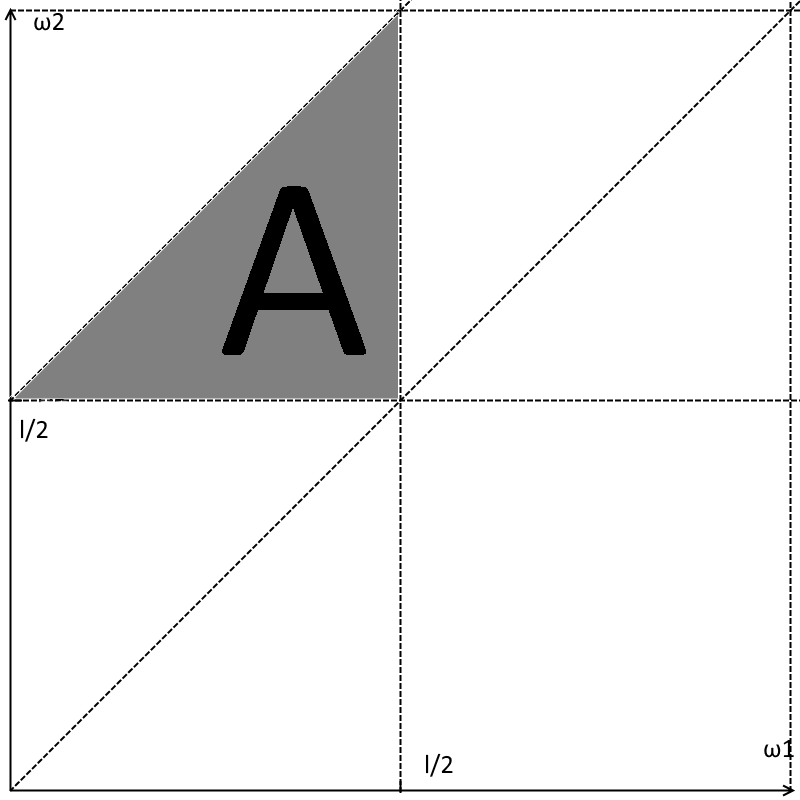
\includegraphics[width=100pt]{triangle.png}
		
		$P(A)=\frac{1}{4}$, from the picture.
	\end{myex}
	
	\newpage\subsection{Laplace Probability Spaces}
	Here is a similar construction, based on the number $|\Omega|$ of elements in $\Omega$.
	\begin{myprop}{}{}
		Let $1\leq|\Omega|<\infty$, $\mathcal{F}=\mathcal{P}(A), P(A)=\frac{|A|}{|\Omega|}\;\forall A\in\mathcal{F}$. Then, $(\Omega, \mathcal{F}, P)$ is a finite probability space called a Laplace probability space.\\
		
		$P$ is discrete uniform distribution on $\Omega$.
		
		\begin{proof}
			Apply Prop. \ref{pr:prob} with $\mu(A)=|A|$ (counting measure).
		\end{proof}
	\end{myprop}
	
	\begin{myrem}{}{}
		For Laplace probability spaces, probability mass function on $\Omega$ is\\
		
		$f(\omega)=P(\{\omega\})=\frac{|\{\omega\}|}{|\Omega|}=\frac{1}{|\Omega|}\;\forall\omega\in\Omega$
		
		so the discrete uniform distribution assigns equal probability $\frac{1}{|\Omega|}$ to each $\omega\in\Omega$.
	\end{myrem}
	
	\begin{myex}{}{}
		\begin{enumerate}
			\item Determine probability of obtaining 1 or 5 when rolling a fair, 6-sided die.
			\begin{align*}
				\Omega&=\{1, \dots, 6\}\\
				\mathcal{F}&=\mathcal{P}(\Omega)\\
				P(A)&=\frac{|A|}{|\Omega|}\;\forall A\in\Omega
			\end{align*}
			
			Let $A=$``rolling 1 or 5"$=\{1, 5\}$. Then, $P(A)=\frac{2}{6}=\frac{1}{3}$.
			\item Determine probability of obtaining a sum of 2 and 7 when rolling the die twice.
			\begin{align*}
				\Omega&=\begin{matrix}
				\{(1, 1), & \dots, & (1, 6),\\
				& \ddots & \\
				(6, 1), & \dots, & (6, 6)\}
				\end{matrix}\\
				\mathcal{F}&=\mathcal{P}(\Omega)\\
				P(A)&=\frac{|A|}{|\Omega|}\;\forall A\in\mathcal{F}
			\end{align*}
			
			So,\\
			
			$P($``sum is 2"$)=\frac{1}{36}$\\
			
			$P($``sum is 7"$)=\frac{6}{36}=\frac{1}{6}$\\
			\item Determine probability of obtaining at least one 6 when rolling 3 times.
			\begin{align*}
				\Omega&=\{(\omega_1, \omega_2, \omega_3) | \omega_i\in\{1, \dots, 6\}\;\forall i\}\\
				\mathcal{F}&=\mathcal{P}(\Omega)\\
				P(A)&=\frac{|A|}{|\Omega|}\;\forall A\in\mathcal{F}
			\end{align*}
			
			So, $P($``at least one 6"$)=1-P($``no 6s"$)=1-(\frac{5}{6})^3=\frac{91}{216}$
		\end{enumerate}
	\end{myex}
	
	\newpage
	\section{Probability Counting Techniques}
	\subsection{Basic Rules}
	
	\begin{myprop}{}{}
		\begin{enumerate}
			\item If $A_1, \dots, A_n$ are pointwise disjoint finite sets, then\\
			$|\bigcup_{i=1}^{n}A_i|=\sum_{i=1}^{n}|A_i|$ (addition rule).
			\item If $A_1, \dots, A_n$ are finite sets, then\\
			$|\prod_{i=1}^{n}A_i|=\prod_{i=1}^{n}|A_i|$ (multiplication rule).
		\end{enumerate}
		
		\begin{proof}
			By induction.
		\end{proof}
	\end{myprop}
	
	\begin{myex}{}{}
		Consider an urn with 5 balls labelled 1, \dots, 5. Determine the probability of obtaining precisely 1 even ball when drawing twice with replacement. Let $\mathbb{E}$ be the set of even integers.
		\begin{align*}
			\Omega&=\begin{matrix}
				\{(1, 1), & \dots, & (1, 5),\\
				& \ddots & \\
				(5, 1), & \dots, & (5, 5)\}
				\end{matrix}\\
			\mathcal{F}&=\mathcal{P}(\Omega)\\
			A&=\{(\omega_1, \omega_2)\in\Omega : \omega_1+\omega_2\notin\mathbb{E}\}\\
			&=A_1\dot\cup A_2
		\end{align*}
		where
		\begin{align*}
			A_1&=\{(\omega_1, \omega_2) : \omega_1\in\mathbb{E}, \omega_2\notin\mathbb{E}\}\\
			A_2&=\{(\omega_1, \omega_2) : \omega_1\notin\mathbb{E}, \omega_2\in\mathbb{E}\}\\
			\therefore P(A)&=\frac{|A|}{|\Omega|}\\
			&=\frac{|A_1|+|A_2|}{|\Omega|}\\
			&=\frac{2*3+3*2}{25}\\
			&=\frac{12}{25}
		\end{align*}
	\end{myex}
	
	\subsection{Urn Models}
	Many counting problems can be associated with drawing k balls from an urn with n balls. Classical models consider drawing:
	\begin{enumerate}[label=(\Roman*)]
		\item With order, with replacement
		\item With order, without replacement
		\item Without order, without replacement
		\item Without order, with replacement
	\end{enumerate}
	
	What are the number of possibilities in each of the four setups?
	\begin{enumerate}[label=(\Roman*)]
		\item
		\begin{align*}
			\Omega_I&=\{(\omega_1, \dots, \omega_k) : \omega_i\in\{1, \dots., n\}, i\in\{1, \dots, k\}\}\\
			&=\prod_{i=1}^k\{1, \dots, n\}\\
			&=\{1, \dots, n\}^k\\
			\Rightarrow|\Omega_I|&=n^k
		\end{align*}
		\begin{myex*}{}{}
			\begin{enumerate}
				\item The number of 53 digit numbers containing only 0-1 is $2^{53}\approx9\cdot10^{15}$.
				\item The number of functions from $A\to B$, where $|A|=k, |B|=n$ is $n^k$.
			\end{enumerate}
		\end{myex*}
		\item
		\begin{align*}
			\Omega_{II}&=\{(\omega_1, \dots, \omega_k) : \omega_i\in\{1, \dots., n\}, \omega_i\neq\omega_j\forall i\neq j\}\\
			\Rightarrow|\Omega_{II}|&=n(n-1)(n-2)\dots(n-k+1)\\
			&=:(n)_k
		\end{align*}
		Where $(n)_k$ is the ``falling factorial" and is read ``n to k factors".
		\begin{myex*}{}{}
			\begin{enumerate}
				\item The number of 3 digit numbers with unique digits in $\{1, \dots, 9\}$ is $(9)_3=9\cdot8\cdot7=504$.
				\item The number of injective functions from $A\to B$, where $|A|=k, |B|=n$ is $(n)_k$.
				\item If $k=n$, then $(n)_k=n!$, and $0!=1!=1$.\\
				$$n!\sim\big(\frac{n}{e}\big)^n\sqrt{2\pi n}$$ (Stirling's formula)
			\end{enumerate}
		\end{myex*}
		\item
		\begin{equation*}
			\Omega_{III}=\{(\omega_1, \dots, \omega_k) : \omega_i\in\{1, \dots, n\}\forall i, \omega_1<\dots<\omega_k\}
		\end{equation*}
		\begin{mydef*}{Equivalence Relation}{}
			An \underline{equivalence relation} $\sim$ is a relation on some set $S$ such that:
			\begin{enumerate}[label=(\roman*)]
				\item $x\sim x$ for all $x\in S$. (reflexive)
				\item $x\sim y\Leftrightarrow y\sim x$ for all $x, y\in S$. (symmetric)
				\item $x\sim y$ and $y\sim z\Rightarrow x\sim z$ for all $x, y, z\in S$. (transitive)
			\end{enumerate}
			An \underline{equivalence class} of some $a\in S$ is $\{x\in S : a\sim x\}$.
		\end{mydef*}
		Now, define an equivalence relation $\sim$ on $\Omega$ via $(\omega_1, \dots, \omega_k)\sim(\omega_1', \dots, \omega_k')$ iff there exists a permutation $\pi : \{1, \dots, k\}\to\{1, \dots, k\}$ such that\\
		$(\omega_1, \dots, \omega_k)\sim(\omega_{\pi(1)}', \dots, \omega_{\pi(k)}')$. Then, $\Omega_{II}$ consists of ordered representations of the equivalence classes of $\sim$, and each such class has n! elements. Thus, $|\Omega_{II}|=|\Omega_{III}|k!$, so $|\Omega_{III}|=\binom{n}{k}$.
		\begin{myex*}{}{}
			\begin{enumerate}
				\item Lotto 6/49 draws 6 from 49 without order and without replacement. Therefore, there are $\binom{49}{6}$ possible outcomes and the chance of some ticket winning is $\frac{1}{\binom{49}{6}}\approx7.15\cdot10^{-8}$
				\item How many subsets of size k does a set of size n have? $\binom{n}{k}$. Therefore,
				$$\sum_{k=0}^n\binom{n}{k}=2^n$$
			\end{enumerate}
		\end{myex*}
		Note that $\binom{n}{k}=\frac{n!}{k!(n-k)!}=\frac{n!}{(n-k)!(n-(n-k))!}=\binom{n}{n-k}$.
		\item Here, we can't simply use (I) and divide by k! (eg. If the $2^{nd}$ ball we draw equals (does not equal) the first, then the permutations don't need to be (do need to be) considered. Identify by distinguishable permutations of $n-1$ ``1" and $k$ ``0".\\
		$\Rightarrow|\Omega_{IV}|=\frac{number\;of\;n-1+k\;symbols}{(number\;of\;permutations\;of\;n-1\;``1"s)(number\;of\;permutations\;of\;k\;``0"s)}=\binom{n-1+k}{k}$\\
		
		Formally, $\Omega_{IV}=\{(\omega_1, \dots, \omega_k) : \omega_i\in\{1, \dots, n\}\;\forall i, \omega_1\leq\dots\leq\omega_k\}$. Note that if $f(\omega_1, \dots, \omega_k)=(\omega_1, \omega_2+1, \dots, \omega_k+k-1)$ is a bijection from $\Omega_{IV}$ to $\Omega_{III}'=\{(\omega_1, \dots, \omega_k) : \omega_i\in\{1, \dots, n+k-1\}\;\forall i, \omega_1<\dots<\omega_k\}$.\\
		$\Rightarrow|\Omega_{IV}|=|\Omega_{III}'|=\binom{n+k-1}{k}$.
		\begin{myex*}{}{}
			\begin{enumerate}
				\item How many possible domino stones are there? A domino has two squares, each of which can be contain 0-6 dots.\\
				$n=7, k=2\Rightarrow\binom{n+k-1}{k}=28$
				\item How many different partial derivatives $\frac{\partial^k}{\partial x_{jk}\dots\partial x_{j1}}f$ of $f\in C^k(\mathbb{R}^n)$ exist?\\
				
				By Scwartz' or Clairaut's theorem, order doesn't matter. Furthermore, we can differentiate with respect to same variable multiple times (so there is replacement).\\
				$\Rightarrow\exists!\binom{n+k-1}{k}$ different partial derivatives.
			\end{enumerate}
		\end{myex*}
	\end{enumerate}
	
	\newpage
	\section{Conditional Probability and Independence}
	\begin{myprop}{}{}
		Let $(\Omega, \mathcal{F}, P)$ be a probability space, and $B\in\mathcal{F} : P(B)>0$. Then, $P(A|B):=\frac{P(A\cap B)}{P(B)}, A\in\mathcal{F}$ is a probability measure on $(\Omega, \mathcal{F})$, called the ordinary conditional probability of A given B. (The vertical bar in the expression $P(A|B)$ means ``given".)
		\begin{proof}~
			\begin{enumerate}[label=(\roman*)]
				\item Let $A\in\mathcal{F}$.
				\begin{align*}
					0&\leq P(A\cap B)\leq P(B)\\
					&\Rightarrow\frac{P(A\cap B)}{P(B)}\leq1\\
					&\Rightarrow P(.|B) : \mathcal{F}\to[0, 1]
				\end{align*}
				\item $P(\Omega|B)=\frac{P(\Omega\cap B)}{P(B)}=\frac{P(B)}{P(B)}=1$
				\item If $\{A_i\}_{i\in\mathbb{N}}\in\mathcal{F}, A_i\cap A_j=\varnothing\;\forall i\neq j$, then
				\begin{align*}
					P(\bigcup_{i=1}^{\infty}A_i|B)&=\frac{P((\bigcup_{i=1}^{\infty}A_i)\cap B)}{P(B)}\\
					&=\frac{\sum_{i=1}^{\infty}P(A_i\cap B)}{P(B)}\\
					&=\sum_{i=1}^{\infty}\frac{P(A_i\cap B)}{P(B)}\\
					&=\sum_{i=1}^{\infty}P(A_i|B)
				\end{align*}
			\end{enumerate}
		\end{proof}
	\end{myprop}
	
	Although $P(A|B)$ is only defined if $P(B)>0$, the convention $P(A|B)P(B)=P(A\cap B)\leq P(B)$ makes sense for any definition of $P(A|B)\in[0, 1]$ if $P(B)=0$.
	\begin{mythm}{Law of Total Probability}{}
		Let $(\Omega, \mathcal{F}, P)$ be a probability space, $\{B_i\}_{i\in\mathbb{N}}\subseteq\mathcal{F}$ be a partition of $\Omega$. That is, $$\Omega=\dot\bigcup_{i=1}^{\infty}B_i, B_i\cap B_j=\varnothing\;\forall i\neq j$$
		Then,
		\begin{align*}
			A\in\mathcal{F}\Rightarrow P(A)&=\sum_{i=1}^{\infty}P(A\cap B_i)\\
			&=\sum_{i=1}^{\infty}P(A|B_i)P(B_i)
		\end{align*}
		\begin{proof}
			\begin{align*}
				A\in\mathcal{F}\Rightarrow P(A)&=P(A\cap\Omega)\\
				&=P(A\cap\bigcup_{i=1}^{\infty}B_i)\\
				&=P(\bigcup_{i=1}^{\infty}(A\cap B_i))\\
				&=\sum_{i=1}^{\infty}P(A\cap B_i)\\
				&=\sum_{i=1}^{\infty}P(A|B_i)P(B_i)
			\end{align*}
		\end{proof}
	\end{mythm}
	
	\begin{myrem}{}{}
		It is often helpful to visualize conditional probabilities in a tree diagram. For example, if $\{A_i\}_{i\in\mathbb{N}}^m, \{B_i\}_{i\in\mathbb{N}}^n\subseteq\mathcal{F}$ are permutations of $\mathcal{F}$,\\
		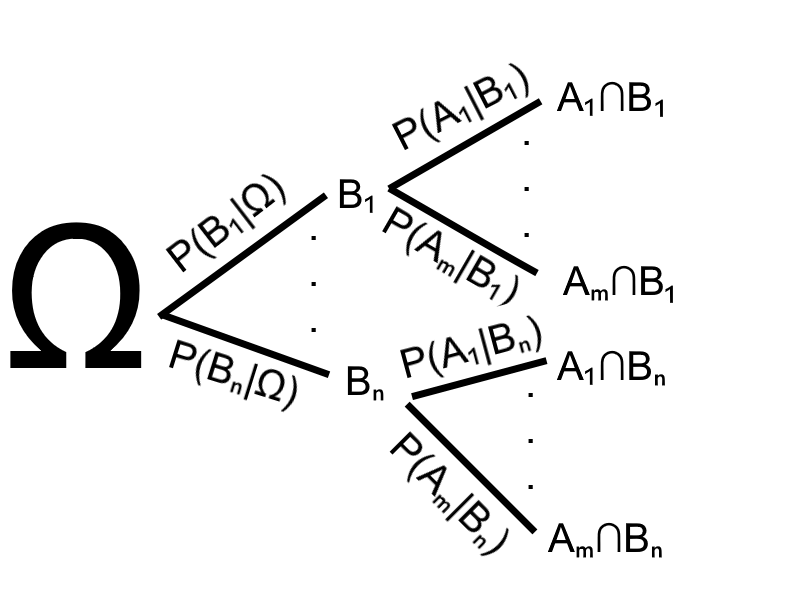
\includegraphics[width=200pt]{tree.png}
		\begin{align*}
			P(A_1\cap B_1)&=P(A_1|B_1)P(B_1)\\
			P(A_m\cap B_1)&=P(A_m|B_1)P(B_1)\\
			P(A_1\cap B_n)&=P(A_1|B_n)P(B_n)\\
			P(A_m\cap B_n)&=P(A_m|B_n)P(B_n)\\\\
			\sum_{i, j=1}^{m, n}P(A_i\cap B_j)&=\sum_{i, j=1}^{m, n}P(A_i|B_j)P(B_j)\\
			&=\sum_{i=1}^m\sum_{j=1}^nP(A_i|B_j)P(B_j)\\
			&=P(\bigcup_{i=1}^mA)\\
			&=P(\Omega)\\
			&=1
		\end{align*}
	\end{myrem}
	
	\begin{myex}{}{}
		\begin{enumerate}
			\item Consider an urn with 2 dice, where $die_1$ has sides (1, 1, 1, 6, 6, 6) and $die_2$ has sides (1, 2, 3, 4, 5, 6). Draw a die at random and roll it. What is $P(``roll\;6")$?
		
			Let $\Omega=\{(1, 1), (1, 6), (2, 1), \dots, (2, 6)\}$, $\mathcal{F}=\mathcal{P}(\Omega)$. Define $P$ as:\\
			\begin{center}
				\begin{tabular}{c|c|c|c|c|c} 
					 $(\omega_1, \omega2)$ & (1, 1) & (1, 6) & (2, 1) & \dots & (2, 6) \\
					 \hline
	$P(\{(\omega_1, \omega_2)\})$ & $\frac{1}{2}\frac{1}{2}=\frac{1}{4}$ & $\frac{1}{2}\frac{1}{2}=\frac{1}{4}$ & $\frac{1}{2}\frac{1}{6}=\frac{1}{12}$ & $\frac{1}{2}\frac{1}{6}=\frac{1}{12}$ & $\frac{1}{2}\frac{1}{6}=\frac{1}{12}$
				\end{tabular}
			\end{center}
			
			Let $A=``Rolling\;6"=\{(\omega_1, \omega_2)\in\Omega : \omega_2=6\}$\\
			$B=``Drawing\;die\;1"=\{(\omega_1, \omega_2)\in\Omega : \omega_1=1\}$
			\begin{align*}
				P(A)&=P(A|B)P(B)+P(A|B^c)P(B^c)\\
				&=\frac{1}{2}\frac{1}{2}+\frac{1}{6}\frac{1}{2}\\
				&=\frac{1}{3}
			\end{align*}
			
			\item Monty Hall problem.\\\\
			Suppose you can choose between 3 doors. Behind one is a car, behind the others are goats. You pick a door, wlog, $door_1$.\\
			The host then, possibly randomly, opens one of the other doors, with a goat behind it. He then gives you a chance to switch to the remaining door. Should you (assuming you want a car more than you want a goat)?\\\\
			Let $\Omega=\{(\omega_1, \omega_2) : \omega_1\in\{1, 2, 3\}, i=1, 2\}$, where $\omega_1$ represents the door containing a car and $\omega_2$ represents the door the host reveals.\\
			Let $\mathcal{F}=\mathcal{P}(\Omega)$\\
			Let $A_i=\{(\omega_1, \omega_2)\in\Omega : \omega_1=i\}, i=1, 2, 3$\\
			$B_j=\{(\omega_1, \omega_2)\in\Omega : \omega_2=j\}, i=2, 3$\\
			
			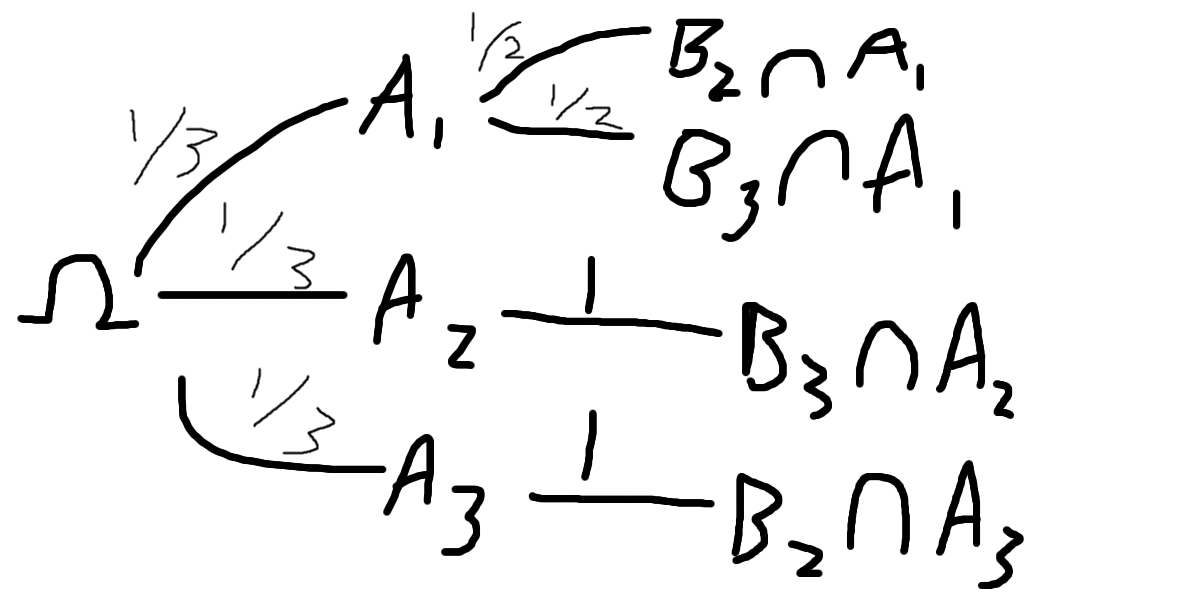
\includegraphics[width=200px]{tree2.png}
			
			\begin{align*}
				\Rightarrow P(A_1\cap B_2) n&=P(B_2|A_1)P(A_1)=\frac{1}{2}\frac{1}{3}=\frac{1}{6}\\
				P(A_1\cap B_3) n&=P(B_3|A_1)P(A_1)=\frac{1}{2}\frac{1}{3}=\frac{1}{6}\\
				P(A_2\cap B_3) n&=P(B_3|A_2)P(A_2)=1\frac{1}{3}=\frac{1}{3}\\
				P(A_3\cap B_2) n&=P(B_2|A_3)P(A_3)=1\frac{1}{3}=\frac{1}{3}\\\\
			\end{align*}
			\[
				\Rightarrow	P(\{(\omega_1, \omega_2)\})=\begin{cases}
					\frac{1}{6} &\mbox{if } (\omega_1, \omega_2)=(1, 2)\\
					\frac{1}{6} &\mbox{if } (\omega_1, \omega_2)=(1, 3)\\
					\frac{1}{3} &\mbox{if } (\omega_1, \omega_2)=(2, 3)\\
					\frac{1}{3} &\mbox{if } (\omega_1, \omega_2)=(3, 2)\\
					0 &\mbox{otherwise}					
			\end{cases}
			\]
			So, $P(\mbox{winning when not switching})=P(\{(\omega_1, \omega_2)\in\Omega : \omega_1=1\})=\frac{1}{6}+\frac{1}{6}=\frac{1}{3}\\
			P(\mbox{winning when switching})=P(\{(2, 3), (3, 2)\})=\frac{1}{3}+\frac{1}{3}=\frac{2}{3}$
			$\therefore$ switching is better.\\
			
			We can also see this from
			\begin{align*}
				P(A_2|B_3)&=\frac{P(A_2\cap B_3)}{P(B_3)}\\
				&=\frac{P(A_2\cap B_3}{P(A_1\cap B_3)+P(A_2\cap B_3)+P(A_3\cap B_3)}\\
				&=\frac{\frac{1}{3}}{\frac{1}{6}+\frac{1}{3}+0}\\
				&=\frac{2}{3}\\
			\end{align*}
			Which also equals $P(A_3|B_2)$ by a similar argument.
		\end{enumerate}
	\end{myex}
	
	\begin{mythm}{Bayes' Theorem}{}
		Let $(\Omega, \mathcal{F}, P)$ be a probability space,\\
		$A\in\mathcal{F}$ such that $P(A)>0$.\\
		Then, $P(B|A)=\frac{P(A|B)P(B)}{P(A)}$ for $A, B\in\mathcal{F}$. Also, if $\{B_i\}_{i\in\mathbb{N}}\subseteq\mathcal{F}$ is a partition of $\Omega$, then
		\begin{align*}
			P(B_i|A)&=\frac{P(A_i|B)P(B_i)}{P(A)}\\
			&=\frac{P(A|B_i)P(B_i)}{\sum_{j=1}^{\infty}P(A|B_j)P(B_j)}
		\end{align*}
		\begin{proof}
			$P(B|A)=\frac{P(B\cap A)}{P(A)}=\frac{P(A\cap B)}{P(A)}=\frac{P(A|B)P(B)}{P(B)}$
		\end{proof}
	\end{mythm}
	
	\begin{myex}{}{}
		A phone sends 0s and 1s (ratio = 3:2) to an antenna. With a certain probability $p\in(0, 1)$, 0s are received wrongly as 1s. With a certain probability $q\in(0, 1)$, 1s are received wrongly as 0s.
		\begin{enumerate}[label=(\alph*)]
			\item Find probability that a 1 is received.
			\item Find probability that a 1 has been sent, given a 1 has been received.
		\end{enumerate}
		\paragraph{Solution.}
		\begin{enumerate}[label=(\alph*)]
			\item Let $\Omega=\{\omega_1, \omega_2) : \omega_i\in\{0, 1\}, i=1, 2\}\\
			\mathcal{F}=\mathcal{P}(\Omega)\\
			S_i=$``i sent"$=\{(i, 0), (i, 1)\}\;i=0, 1\\
			R_i=$``i received"$=\{(0, i), (1, i)\}\;i=0, 1$. Then,
			\begin{align*}
				P(R_1)&=P(R_1|S_0)P(S_0)+P(R_1|S_1)P(S_1)\\
				&=p\frac{3}{5}+(1-q)\frac{2}{5}\\
				&=0.6p+0.4(1-q)
			\end{align*}
			\item
			\begin{align*}
				P(S_1|R_1)&=\frac{P(R_1|S_1)P(S_1)}{P(R_1)}\\
				&=\frac{0.4(1-q)}{0.6p+0.4(1-q)}
			\end{align*}
			From (a).
		\end{enumerate}
	\end{myex}
	
	
	If $P(A|B)$ does not depend on $B$, then $$P(A\cap B)=P(A|B)P(B)=P(A)P(B)$$
	These events are independent.
	\begin{mydef}{Independence}{}
		Let $(\Omega, \mathcal{F}, P)$ be a probability space. Then
		\begin{enumerate}[label=(\roman*)]
			\item $A_1, A_2\in\mathcal{F}$ are \underline{independent} if $P(A_1\cap A_2)=P(A_1)P(A_2)$.
			
			\item $A_1, \dots, A_n\in\mathcal{F}$ are independent if $P(\bigcap_{i=1}^{n}A_i)=\prod_{i=1}^{n}P(A_i)$.
			
			\item $\mathcal{A}_1, \dots, \mathcal{A}_n\subseteq\mathcal{F}$ are independent if $A_1, \dots, A_n$ are independent for all $A_i\in\mathcal{A}_i$.
			
			\item $\{A\}\subseteq\mathcal{F}$ is independent if $A_{i_1}, \dots, A_{i_n}$ are independent for all $\{i_1, \dots, i_n\}$. That is, if all finite subsets are independent.
		\end{enumerate}
	\end{mydef}
	
	\newpage
	\section{Random Variables and Distributions}
	When predicting outcomes of experiments, it is useful to consider mappings $X : \Omega\to\Omega'$ for some measurable set $(\Omega', \mathcal{F}')$, often $(\R, \mathcal{B}(\R))$ or $(\R^d, \mathcal{B}(\R^d))$.
	
	\subsection{Random Variables}
	\begin{mydef}{Preimage}{}
		The \underline{preimage} of $X : \Omega\to\Omega'$ is defined by $X^{-1}(A')=\{\omega\in\Omega : X(\omega)\in A'\}, A'\subseteq\Omega'$.
	\end{mydef}
	
	\begin{mylem}{}{}
		\begin{enumerate}[label=(\roman*)]
			\item $X^{-1}(\varnothing)=\varnothing, X^{-1}(\Omega')=\Omega$
			\item $(X^{-1}(A'))^c=X^{-1}(A'^c)\;\forall A'\subseteq\Omega'$
			\item
			$\bigcup_{i\in I}X^{-1}(A_i')=X^{-1}(\bigcup_{i\in I}A_i'),\\
			\bigcap_{i\in I}X^{-1}(A_i')=X^{-1}(\bigcap_{i\in I}A_i')$
		\end{enumerate}
		
		If $\mathcal{F}$ is a $\sigma$-algebra on $\Omega'$, then $\sigma(X):=\{X^{-1}(A') : A'\in\mathcal{F}\}$ is a $\sigma$-algebra on $\Omega$, the $\sigma$-algebra generated by $X$.
		
		\begin{proof}~
			\begin{enumerate}[label=(\roman*)]
				\item ~
				\item
				\begin{align*}
					&\omega\in(X^{-1}(A'))^c\\
					\Leftrightarrow&\omega\notin X^{-1}(A')\\
					\Leftrightarrow&X(\omega)\notin A'\\
					\Leftrightarrow&X(\omega)\in A'^c\\
					\Leftrightarrow&\omega\in X^{-1}(A'^c)
				\end{align*}
				\item Similar to (ii).
			\end{enumerate}
		\end{proof}
	\end{mylem}
	
	\begin{mydef}{}{}
		Let $(\Omega, \mathcal{F}), (\Omega', \mathcal{F}')$ be measurable. Then, $X : \Omega\to\Omega'$ is called \underline{$((\mathcal{F}, \mathcal{F}')-)$ measurable} if $\sigma(X)\subseteq\mathcal{F}$. I.e. $X^{-1}(A')\in\mathcal{F}\;\;\forall A'\in\mathcal{F}$.\\
		
		If $(\Omega', \mathcal{F}')$ is $(\R, \mathcal{B}(\R))$ or $(\R^d, \mathcal{B}(\R^d))$, $X$ is called a \underline{random variable} $(\omega)$ or \underline{random vector} in this case.
	\end{mydef}
	\newpage
	
	\begin{myex}{}{ex1}
		\begin{enumerate}
			\item Let $(\Omega, \mathcal{F})$ be measurable and $V\subseteq\Omega : V\notin\mathcal{F}$ be a non-measurable (Vitali) set. Then, $X : \Omega\to\R$ (so $(\Omega', \mathcal{F}')=(\R, \mathcal{B}(\R))$) with \[
				X(\omega)=1_v(\omega)=\begin{cases}
					1 \mbox{ if } \omega\in V\\
					0 \mbox{ if } \omega\notin V\\			
			\end{cases}
			\]
			is a non-measurable function since $$X^{-1}((\frac{1}{2}, 1])=\{\omega\in\Omega : X(\omega)\in(\frac{1}{2}, 1]\}=\{\omega\in\Omega : X(\omega)=1\}=V\notin\mathcal{F}$$
			
			\item If $\Omega\neq\varnothing$, no non-constant $X^- : \Omega\to\mathbb{R}$ is $(\{\varnothing, \Omega\}, \mathcal{B}(\mathbb{R}))$-measurable.
			
			\item If $(\Omega, \mathcal{F})$ is a measurable space, the following functions from $\Omega\to\R$ are measurable:
			\begin{enumerate}[label=(\roman*)]
				\item Let $c\in\R, X=c$. Then,
				\begin{align*}
					X\inv(B)&=\begin{cases}
						\Omega,&c\in\mathcal{B}\\
						\varnothing,&c\notin\mathcal{B}
					\end{cases}\\
					\Rightarrow\sigma(X)&=\{\varnothing, \Omega\}\subseteq\mathcal{F}
				\end{align*}
				for $B\in\mathcal{B}(\Omega)$.
				
				\item Let $A\in\mathcal{F}, X=\mathbbm{1}_A$. Then,
				\begin{align*}
					X\inv(B)&=\begin{cases}
						\Omega,&0\in B\mbox{ and }1\in B\\
						A,&0\in B\mbox{ and }1\notin B\\
						A^c,&0\notin B\mbox{ and }1\in B\\
						\varnothing,&0\notin B\mbox{ and }1\notin B\\
					\end{cases}\\
					\Rightarrow\sigma(X)&=\{\varnothing, A, A^c, \Omega\}\subseteq\mathcal{F}
				\end{align*}
				
				\item Let $\{A_i\}_{i\in\{1, \dots, n\}}\subseteq\mathcal{F}$ be a partition of $\Omega$, and $$X_n=\sum_{i=1}^nx_i\mathbbm{1}_{A_i}$$ for $x_i\neq x_j\;\forall i\neq j$. Then, as in parts (i) and (ii), we obtain $$\sigma(X_n)=\{\bigcup_{i\in I}A_i : I=\{1, \dots, n\}\}\subseteq\mathcal{F}$$
			\end{enumerate}
		\end{enumerate}
	\end{myex}
	
	\begin{myrem}{}{}
	    \begin{enumerate}
	        \item We typically write $X$ instead of $X(\omega)$. For example, $X=1_A$ instead of $X(\omega)=1_A(\omega)$. This is to not confuse the study of $X$ (a function) with $X(\omega)$ (a single value often denoted $x$, referred to as a ``realization" of $X$, after an experiment has been conducted and $\omega$ (state of the world) is known).
	        
	        \item Part 3 (iii) of \ref{ex:ex1} hints at the fact that we can study sequences of $x_1, \dots, x_n, \dots$. Such sequences play a major role in major limiting results.\\
	        
	        Random variables $X_n$ as in (iii) are called simple random variables, and are the building blocks of defining an integral $EX=\int_\Omega X(\omega)dP(\{\omega\})$ known as ``expectation of X" through a process called algebraic induction.
	        
	        \item One can show measurability is preserved by many operations, eg compositions of measurable functions are measurable. Also 
	        \begin{align*}
	        	\inf_{k\geq n}&X_k\\
	        	\sup_{k\geq n}&X_k\\
	        	\lim_{n\to\infty}\inf &X_n\\
	        	\lim_{n\to\infty}\sup &X_n\\
	        	\lim_{n\to\infty}&X_n
	       	\end{align*} all preserve measurability. Continuous $X$ are measurable and whenever we use such operations, assume resulting mappings to be measurable.
	       	
	       	\item One can show random vectors are vectors of random variables. We typically write random vectors as $\underline{X}=(X_1, \dots, X_d)$ where $X_1, \dots, X_d$ are random variables.
	    \end{enumerate}
	\end{myrem}
	
	\begin{myprop}{}{}
		If $(\Omega, \mathcal{F}, P)$ is a probability space, $(\Omega', \mathcal{F}')$ a measurable space, $X : \Omega\to\Omega'$ a measurable function, then $$P_X=P\circ X\inv$$ is a probability measure on $(\Omega', \mathcal{F}')$, called the distribution of $X$ (or ``image measure of $P$ with respect to $X$" or ``push-forward measure").
		
		\begin{proof}
			Check the three properties of probability measures.
			\begin{enumerate}[label=(\roman*)]
				\item $P_X : \mathcal{F}'\to[0, 1]$
				
				\item 
				\begin{align*}
					P_X(\Omega')&=P(X\inv(\Omega'))\\
					&=P(\Omega)\\
					&=1
				\end{align*}
				
				\item
				\begin{align*}
					\{A_i\}_{i\in\mathbb{N}}&\subseteq\mathcal{F}', A_i'\cap A_j'=\varnothing \mbox{ for }i\neq j\\
					\Rightarrow P_X(\bigcup_{i=1}^{\infty}A_i')&=P(X\inv(\bigcup_{i=1}^{\infty}A_i'))\\
					&=P(\bigcup_{i=1}^{\infty}X\inv(A_i'))\\
					&=\sum_{i=1}^{\infty}P(X\inv(A_i'))\\
					&=\sum_{i=1}^{\infty}P_X(A_i')
				\end{align*}
			\end{enumerate}
		\end{proof}
	\end{myprop}
	
	\begin{myrem}{}{}
		\begin{enumerate}
			\item $P_X$ assigns probabilities to events involving measurable $X$ since $X\inv(A')\in\mathcal{F}$ for $A'\in\mathcal{F}'$ and $P$ assigns probabilities to such events.
			
			\item We often write
			\begin{align*}
				P(X\in A')&:=P(\{\omega\in\Omega : X(\omega)\in A'\})\\
				&=P(X\inv(A'))\\
				&=P_X(A')
			\end{align*}
			for $A'\in\mathcal{F}'$.
			
			\item If $X$ is a random variable, distribution of $X$ is a Borel probability measure on $\R$. We call
			\begin{align*}
				F(X)&:=P_X((-\infty, x])\\
				&=P(x\in(-\infty, x])
				&=P(\{\omega\in\Omega : X(\omega)\leq x\})
			\end{align*}
			for $x\in\R$ the distribution function (df) of $X$, and write $X\sim F$. For $P(X\in(-\infty, x])$, we write $P(X\leq x)$, so $X\sim F$ iff $F(x)=P(X\leq x)$ for $x\in\R$.
		\end{enumerate}
	\end{myrem}
	
	The following result characterizes all distribution functions on $\R$.
	
	\begin{mythm}{}{5.8}
		$F : \R\to[0, 1]$ is the distribution function of a unique Borel probability measure $P_F$ on $\R$ iff:
		\begin{enumerate}[label=(\roman*)]
			\item $F(-\infty)=\lim_{x\downarrow-\infty}F(x)=0$ and $F(\infty)=\lim_{x\uparrow\infty}F(x)=1$.
			
			\item $F$ is increasing.
			
			\item $F$ is right continuous.
		\end{enumerate}
		Here, $P_F$ is $P_X$ for $X\sim F$.
		
		\begin{proof}
			$(\Rightarrow)$ Suppose $F : \R\to[0, 1]$ is the distribution function of a unique Borel probability measure $P_F$ on $\R$. Then,\\
			\begin{enumerate}[label=(\roman*)]
				\item
				\begin{align*}
					F(-\infty)&=\lim_{n\to\infty}F(-n)\\
					&=\lim_{n\to\infty}P_F((-\infty, -n ])\\
					&=P_F(\bigcap_{n=1}^{\infty}(-\infty, -n])\mbox{ by continuity from above}\\
					&=P_F(\varnothing)\\
					&=0
				\end{align*}
				Also,
				\begin{align*}
					F(\infty)&=\lim_{n\to\infty}F(n)\\
					&=\lim_{n\to\infty}P_F((-\infty, n])\\
					&=P_F(\bigcup_{i=1}^{\infty}(-\infty, n])\mbox{ by continuity from below}\\
					&=P_F(\R)\\
					&=1
				\end{align*}
				
				\item If $x, y\in\R$ such that $x<y$ then $F(x)=P_F((-\infty, x])\leq P_F((-\infty, y])=F(y)$ since $(-\infty, x]\subseteq(-\infty, y]$.
				
				\item Let $\{h_n\}$ be a sequence such that $h_n\downarrow0$ as $n\to\infty$. Then,
				\begin{align*}
					\lim_{n\uparrow\infty}F(x+h_n)&=\lim_{n\uparrow\infty}P_F((-\infty, x+h_n])\\
					&=P_F(\bigcap_{i=1}^{\infty}(-\infty, x+h_n])\\
					&=P_F((-\infty, x])\\
					&=F(x)
				\end{align*}
				for $x\in\R$.\\
				
				$(\Leftarrow)$ By theorem \ref{th:righ}, (ii) and (iii) imply there exists exactlt one Borel measure $\mu_F$ on $\R$ such that $\mu_F((a, b])=F(b)-F(a)$ for $a\leq b$. Thus,
				\begin{align*}
					\mu_F(\R)&=\lim_{n\to\infty}\mu_F((-n, n])\\
					&=\lim_{n\to\infty}(F(-n)-F(n))\\
					&=1
				\end{align*}
				so $\mu_F$ is a probability measure on $\R$. Its distribution function is $F$ since for all $x\in\R, n\in\N$ such that $n>-x$, $\mu_F((-n, x])=F(x)-F(-n)$ which implies
				\begin{align*}
					F(x)&=\lim_{n\to\infty}(\mu_F((-n, x])+F(-n))\\
					&=\mu_F((-\infty, x])
				\end{align*}
				by continuity from below. So $\mu_F$ is the $P_F$ as claimed. (Also $P_F$ satisfies $P_F((a, b])=F(b)-F(a)$ for all $a\leq b$.)
			\end{enumerate}
		\end{proof}
	\end{mythm}
	
	\begin{myrem}{}{c5i9}
		$(\Rightarrow)$ implies any distribution function $F$ has those properties.\\
		
		$(\Leftarrow)$ implies any such $F$ induces a unique distribution with distribution function $F$. Here are some examples of such distributions.
		
		\begin{enumerate}
			\item $F(x)=\min\{\max\{x, 0\}, 1\}$ for $x\in\R$ is the distribution function of the \underline{standard uniform distribution, $U(0, 1)$}.
			
			\item $F(x)=\int_{-\infty}^x\frac{1}{\sqrt{2\pi\sigma^2}}e^{\frac{-1}{2}(\frac{z-\mu}{\sigma})^2}dz$ for $x, \mu, \sigma\in\R, \sigma>0$ is the distribution function of the \underline{normal distribution, $N(\mu, \sigma^2)$}
			
			\item $F(x)=(1-p)\mathbbm{1}_{[0, \infty)}(x)+p\mathbbm{1}_{[1, \infty)}(x)$ for $x\in\R, p\in[0, 1]$ is the distribution function for the \underline{Bernoulli distribution, $B(1, p)$}.\\
			
			How do we construct $X\sim F$ in this case?
		\end{enumerate}
	\end{myrem}
	
	\begin{mydef}{}{}
		If $F : \R\to\R$ is increasing, the \underline{generalized inverse $F^-$} of $F$ is defined by $F^-(y)=\inf\{x\in\R : F(x)\geq y\}$ for $y\in\R$.\\
		
		If $F$ is a distribution function, $F^-$ is the \underline{quantile function} of $F$. 
	\end{mydef}
	
	\begin{myrem}{}{}
		\begin{enumerate}
			\item Sketch:
			
			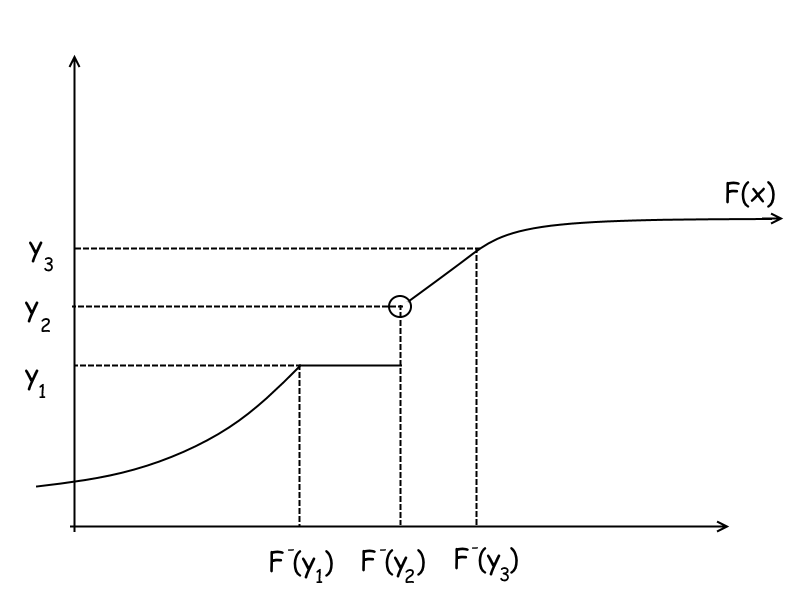
\includegraphics[scale=.5]{graph1.png}
			
			\item Some facts:
			\begin{itemize}
				\item If $F$ is strictly increasing and continuous, then $F^-=F\inv$, the ordinary inverse.
				\item $F^-$ is increasing and left-continuous.
				\item One can often work with $F^-$ as $F\inv$ (which we will do), but be careful when it matters, such as in the sketch where $F(F^-(y_2))>y2$.
			\end{itemize}
			Quantile functions allow us to answer remark \ref{re:c5i9}.
		\end{enumerate}
	\end{myrem}
	
	\begin{myprop}{}{5.12}
		If $F : \R\to[0, 1]$ satisfies (i), (ii), (iii) of theorem \ref{th:5.8} then there is a probability space $(\Omega, \mathcal{F}, P)$ and random variable $X : \Omega\to\R$ such that $X\sim F$.
		
		\begin{proof}
			Consider $(\Omega, \mathcal{F}, P)=((0, 1), \bar{\mathcal{B}}((0, 1)), \lambda)$ and $X(\omega):=F^-(\omega)$ for $\omega\in\R$. Then,
			\begin{align*}
				P(X\leq x)&=P(\{\omega\in\Omega : X(\omega)\leq x\})\\
				&=P(\{\omega\in\Omega : \omega\leq F(x)\})\\
				&=P((0, F(x))=\lambda((0, F(x))\\
				&=F(x)
			\end{align*}
			for all $x\in\R$. We can also use the notation $P_X$ for $P_F$.
		\end{proof}
	\end{myprop}
	
	Proposition \ref{pr:5.12} can be exploited to generate (pseudo-)random numbers. Pseudorandom numbers are numbers which resemble realizations of $X\sim F$ on a computer based on following a result known as inversion method for sampling (generating random numbers). Note that there are various ways to sample from $U(0, 1)$ (distribution function is $F_U(x)=x\;\forall x\in[0, 1]$) on a computer.
	
	\begin{myprop}{}{5.13}
		Let $F$ be a distribution function, $U\sim U(0, 1)$. Then $X : F^-(U)\sim F$.
		
		\begin{proof}
			\begin{align*}
				P(X\leq x)&=P(F^-(U)\leq x)\\
				&=P(U\leq F(x))\\
				&=F_U(F(x))\mbox{ since $U\sim U(0, 1)$}\\
				&=F(x)
			\end{align*}
		\end{proof}
	\end{myprop}
	
	\begin{myrem}{}{}
		\begin{enumerate}
			\item If $X\sim F$, proof of theorem \ref{th:5.8} $(\Leftarrow)$ implies that
			\begin{align*}
				P(X\in(a, b])&=P_X((a, b])\\
				&=P_F((a, b])\\
				&=F(b)-F(a)
			\end{align*}
			
			\item If $X\sim F$, then 
			\begin{align*}
				P(X=x)&=P(X\in\bigcap_{i=1}^{\infty}(x-\frac{1}{n}, x])\\
				&=\lim_{n\to\infty}P(X\in(x-\frac{1}{n}, x])\\
				&=F(x)-\lim_{n\to\infty}F(x-\frac{1}{n})\\
				&=F(x)-F(x-)
			\end{align*}
			for $x\in\R$.
			\begin{itemize}
				\item If $F$ is continuous, then $P(X=x)=0$.
				\item If $F$ is constant over $(a, b]$, then $P(x\in(a, b])=F(b)-F(a+)=0$.
				\item If $F$ jumps in $x$, then $P(X=x)=F(x)-F(x-)$, so the probability equals the jump height of $F$ in $x$.
				\item Note that in each ``jump gap" $(F(x-), F(x))$ is a rational number and since $F$ is increasing, they are all distinct. Therefore, the number of jumps is at most equal to the number of rationals, so distribution functions can have at most countably many jumps.
			\end{itemize}
		\end{enumerate}
	\end{myrem}
	
	\begin{mydef}{}{}
		Let $X$ be a random variable, with distribution $P_X$ and distribution function $F$.
		\begin{enumerate}
			\item $X(P_X, F)$ is a \ul{discrete random variable (discrete distribution, discrete distribution function)} if there is $S=\{x_1, \dots, x_n, \dots\}\subseteq \R$ such that $P(X\in S)=1$. Equivalently, if $F$ is a step function or if $\mbox{range}(F):=\{F(x) : x\in\R\}$ is at most countable.
			
			\item $X(P_X, F)$ is a \ul{continuous(ly distributed) random variable (continuous distribution, continuous distribution function)} if $F$ is continuous.
			
			\item $X(P_X, F)$ is an \ul{absolutely continuous(ly distributed) random variable (absolutely continuous distribution, absolutely continuous distribution function)} if $$F(x)=\int_{-\infty}^{x}f(z)dz$$ for some function $f(z) : \R\to[0, \infty)$ which is integrable, such that $\int_{-\infty}^{\infty}f(z)dz=1$. Then, $f$ is called the density of $X(P_X, F)$.
		\end{enumerate}
	\end{mydef}
	
	\begin{myrem}{}{}
		\begin{enumerate}
			\item Not all distribution functions $F$ are discrete, continuous or absolutely continuous. They can have mixed type, that is, be discrete on one nonzero interval and continuous on another. Here is a sketch of one such distribution function.\\
			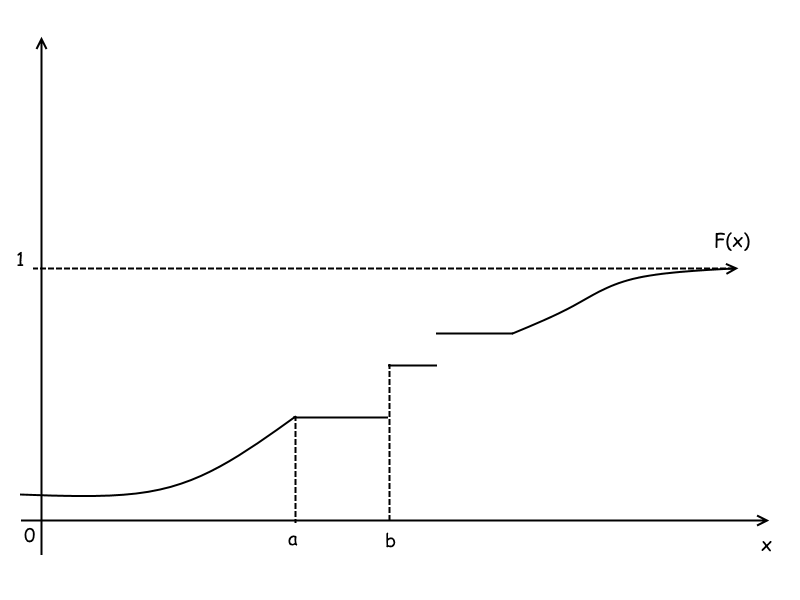
\includegraphics[scale=.5]{graph2.png}
			
			If $X\sim F$, then
			\begin{align*}
				P(x\in(a, b])&=F(b)-F(a)=\mbox{ ``jump height"}\\
				P(x=a)&=F(a)-F(a-)=0\\
				P(x\in(a, b))&=0
			\end{align*}
			
			\item If $F$ is differentiable everywhere on $\R$, $F'$ is integrable, and the fundamental theorem of calculus implies $F$ is absolutely continuous with density $f=F'$.\\
			
			Every absolutely continuous function $F$ is continuous since
			\begin{align*}
				|F(x_h)-F(x)|&=|\int_{x}^{x+h}f(z)dz|\\
				&\leq\int_{x}^{x+h}f(z)dz\\
				&\leq M\int_{x}^{x+h}1dz\mbox{ for some $M\in\R$}\\
				&=M(x+h-x)\\
				\Rightarrow\lim_{h\to0}Mh=0
			\end{align*}
			which implies continuity. Also if $X\sim F$ then $P(X=x)=0$ for all $x\in\R$. Hence $P(X=x)\neq f(x)$ in general. However,
			\begin{align*}
				P(X\in(x-\varepsilon, x])&=F(x)-F(x-\varepsilon)\\
				&=\int_{x-\varepsilon}^{x}f(z)dz\\
				&\approx\varepsilon f(x)
			\end{align*}
			for small $\varepsilon>0$. (interpolation of densities)
			\newpage
			
			\item Not all continuous distribution functions are absolutely continuous. Here is an example of a distribution function which is continuous but not absolutely continuous.
			
			For each $x=\sum_{i=1}^{\infty}a_i3^{-i}\in C$ where $a_i\in\{0, 2\}$ and $C$ is the Cantor set, define $F(x):=\sum_{i=1}^{\infty}\frac{a_i}{2}2^{-i}$. That is, a base 2 expansion of a unique number in $[0, 1]$. Thus $F$ maps $C\to[0, 1]$. Now extend the domain such that $F$ is constant in intervals missing from $C$.
			
			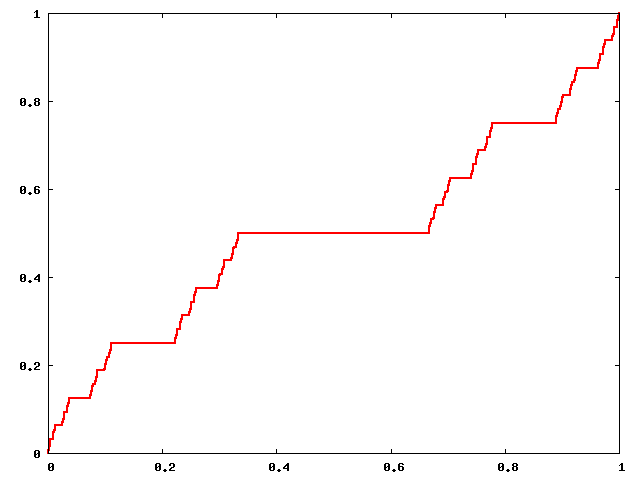
\includegraphics[scale=.5]{devil.png}
			
			So $F$ is increasing, $\mbox{range}(F)=[0, 1]$, and $F$ is continuous. This function is also called Cantor's distribution or the devil's staircase. Since $F$ is constant on $[0, 1]\backslash C$, a density candidate of $F$ would have to be 0 on $[0, 1]\backslash C$. Let $f$ be such a density  candidate. Then,
			\begin{align*}
				\int_{[0, 1]}f(z)dz&=\int_Cf(z)dz+\int_{[0, 1]\backslash C}f(z)dz\\
				&=0\neq1
			\end{align*}
			which shows $F$ is not absolutely continuous.
			
			\item For probability mass functions or densities, always provide a domain. For example $f(x)=\frac{1}{c}$ is a density on $[0, c]$ (namely $U(0, c)$) but not on $[0, \infty)$ since $\int_{0}^{\infty}\frac{1}{c}\neq1$ for all $c\in\R$.
		\end{enumerate}
	\end{myrem}
	
	\begin{myex}{}{5.17}
		\begin{enumerate}
			\item Let $X\sim U(0, 1)\Rightarrow F(x)=P(X\leq x)=x$ for $x\in[0, 1]$. For any pairwise disjoint intervals $(a_i, b_i]\subseteq[0, 1], i\in\N$ with $\sum_{i=1}^{\infty}(b_i-a_i)=h$, we have $P(X\in\sum_{i=1}^{\infty}(a_i, b_i])=h$ by $\sigma$-additivity.
			
			In particular, the probability of $X$ to fall in an interval length $h$ is $h$. This can also be seen from the density, $f(x)=F'(x)=1$ for $x\in(0, 1]$ since $P(X\in(x, x+h])=\int_x^{x+h}f(z)dz=x+h-x=h$.
			
			\item Let $X\sim N(\mu, \sigma^2)$. Then, $F(x)=\int_{-\infty}^x\frac{1}{\sqrt{2\pi\sigma^2}}e^{\frac{-1}{2}(\frac{z-\mu}{\sigma})^2}dz$ and the density candidate is\\
			$f(x)=\frac{1}{\sqrt{2\pi\sigma^2}}e^{\frac{-1}{2}(\frac{z-\mu}{\sigma})^2}$. It can be shown that this is indeed a density but it's just calculus and not on the test and fuck copying that proof into \LaTeX.\\
			
			A random number generator from $N(\mu, \sigma^2)$ can be done with inversion based method based on fast and accurate approximation of $F^-$.
		\end{enumerate}
	\end{myex}	
	
	\subsection{Random Vectors}
	Many notions introduced so far can be extended to random vectors $\underline{X}=(X_1, \dots, X_d)$.
	
	\begin{mydef}{}{}
		Let $(\Omega, \mathcal{F}, P)$ be a probability space, $\underline{X}=(X_1, \dots, X_d)$ a random vector. Then $P_{\underline{X}}=P\circ\underline{X}\inv$ (with $$P_{\underline{X}}(B)=P(\underline{X}\inv(B))=P(\{\omega\in\Omega : \underline{X}(\omega)\in B\})$$ for $B\in\mathcal{B}(\R)$) is called the \underline{distribution of \underline{X}} (a Borel probability measure on $\R^d$) and
		\begin{align*}
			F(\underline{x})&:=P_{\underline{X}}((-\infty, x])\\
			&=P(\underline{X}\in(-\underline{\infty}, \underline{x}])\\
			&=P(\{\omega\in\Omega : X(\omega)\leq\underline{x}\})\\
			&=P(\{\omega\in\Omega : X_j(\omega)\leq x_j\;\forall j=1, \dots, d\})\\
			&=P(\bigcap_{j=1}^{d}\{\omega\in\Omega : X_j(\omega)\leq x_j\})\\
		\end{align*}
		for $\underline{X}=(x_1, \dots, x_d)\in\R^d$ is the distribution function of \underline{X}, as before. We write $\underline{X}\sim F$ in this case, and write $P(\underline{X}\leq\underline{x})$ or $P(X_1\leq x_1, \dots, X_d\leq x_d)$ for $P(\underline{X}\in(-\underline{\infty}, \underline{x}])$.\\
		
		Thus, $X\sim F\Leftrightarrow F(\underline{x})=P(\underline{X}\leq\underline{x})$ for all $\underline{x}\in\R^d$.\\
		
		We call
		\begin{align*}
			F_j(x_j)&=P(X_j\leq x_j)\\
			&=P(X_1\leq\infty, \dots, X_{j-1}\leq\infty, X_j\leq x_j, X_{j+1}\leq\infty, \dots, X_d\leq\infty)\\
			&=F(\infty, \dots, \infty, x_j, \infty, \dots, \infty)
		\end{align*}
		the j-th margin of $F$ or the j-th marginal distribution function of \underline{X}.
	\end{mydef}
	
	Similar to theorem \ref{th:c5i8} (based on remark \ref{re:1.24} (1)), we obtain this characterization of all distribution functions $F$.
	
	\begin{mythm}{}{}
		A function $F : \R^d\to[0, 1]$ is the distribution function of a unique Borel probability measure $P_F(=P_X)$ on $\R^d$ iff:
		\begin{enumerate}[label=(\roman*)]
			\item $\lim_{x_j\to-\infty}F(\underline{x})=0$ for at least one $j=1, \dots, d$ and $\lim_{\underline{x}\uparrow\underline{\infty}}F(\underline{x})=1$.
			
			\item $F$ is d-increasing, that is, $\Delta_{(\underline{a}, \underline{b}]}F\geq0$ for all $a\leq b$ (see remark \ref{re:1.24}).
			
			\item $F$ is right continuous: $\lim_{\underline{h}\downarrow\underline{0}}F(\underline{x}+\underline{h})=F(\underline{x})$ for all $\underline{x}\in\R^d$.
		\end{enumerate}
		
		If we have a distribution function $F$, with $X\sim F$, we have $\Delta_{(\underline{a}, \underline{b}]}F=\mu_F((\underline{a}, \underline{b})=P_X(\underline{a}, \underline{b}])=P(x\in(\underline{a}, \underline{b}])$. So, the F-volume of $(\underline{a}, \underline{b}]$ is the probability of $x\in(a_j, b_j]$ for all $j=1, \dots, d$. This probability can be computed as in remark \ref{re:1.24} (2).
	\end{mythm}
	
	\begin{mydef}{}{}
		Let $\underline{X}=(X_1, \dots, X_d)$ be a random vector with distribution $P_X$ and distribution function $F$.
		\begin{enumerate}
			\item $\underline{X}(P_{\underline{X}}, F)$ is \ul{discrete (discrete distribution, discrete df)} if there exists $S=\{\underline{x}_1, \underline{x}_2, \dots\}\subseteq \R^d$ such that $P(\underline{X}\in S)=1$. Alternatively, if $F$ is a step function. Or, if $\mbox{range}(F):=\{F(\underline{x}) : \underline{x}\in \R^d\}$ is at most countable. In this case, $f(\underline{x}_i)=P(\underline{X}=\underline{x}_i)$ for $i\in\N$ is the probability mass function of $\underline{X}(P_{\underline{X}}, F)$.
			
			\item $\underline{X}(P_{\underline{X}}, F)$ is a \ul{continuously distributed random vector (continuous distribution, continuous df)} if $F$ is continuous.
			
			\item $\underline{X}(P_{\underline{X}}, F)$ is an \ul{absolutely continuous random vector (abs. cont. distribution, abs. cont. df)} if $$F(\underline{x})=\int_{-\infty}^{x_1}\dots\int_{-\infty}^{x_d}f(z_1, \dots, z_d)dz_1\dots dz_d$$ for all $\underline{x}\in\R^d$, for some $f : \R^d\to[0, \infty)$ such that $$\int_{-\infty}^{\infty}\dots\int_{-\infty}^{\infty}f(z_1, \dots, z_d)dz_1\dots dz_d=1$$.				\end{enumerate}
			
		In this case we call $f$ the \ul{(joint) density} of $\underline{X}(P_{\underline{X}}, F)$.
	\end{mydef}
	
	\begin{myrem}{}{}
		\begin{enumerate}
			\item If $F$ is abs. cont., then
				\begin{align*}
					F_j(x_j)&=F(\infty, \dots, \infty, x_j, \infty, \dots, \infty)\\
					&=\int_{-\infty}^{x_j}\int_{-\infty}^{\infty}\dots\int_{-\infty}^{\infty}f(z_1, \dots, z_d)
				\end{align*}
				
				which implies $F_j$ is abs. cont. with density
				\begin{align*}
					f_j(x_j)&=\frac{d}{dx_j}F_j(x_j)\\
					&=\int_{-\infty}^{\infty}\dots\int_{-\infty}^{\infty}f(z_1, \dots, z_{j-1}, x, z_{j+1}, z_d)dz_1\dots dz_{j-1}dz_{j+1}\dots dz_d
				\end{align*}
				
				being the j-th marginal density of $F$. So for $j\in\{1, \dots, d\}$, the j-th margin $F_j$ of $F$ can be obtained by taking limits $(X_k\to\infty\;\forall k\neq j)$ and its density $f_j$ by integrating out the joint density of $f$ with respect to all components except the j-th.
				
			\item We have just shown if $F$ is abs. cont., so are its margins. The converse is not true in general.
		\end{enumerate}
	\end{myrem}
	
	\section{Independence and dependence}
	
	Independence is the most crucial assumption in stochastic models and results.
	
	\begin{mydef}{}{}
		Let $(\Omega, \mathcal{F}, P)$ be a probability space, $(\Omega', \mathcal{F}')$ a measurable space, and $X_i : \Omega\to\Omega'$ be $(\mathcal{F}, \mathcal{F}')-$measurable for all $i\in I\subseteq\R$.\\
		
		Then, $X_i, i\in I$ are independent if $\sigma(X_i), i\in I$ are independent. That is, if $$X_{i_1}\inv(A_{i_1}'), \dots, X_{i_n}\inv(A_{i_n}')$$ are independent for all $$A_{i_1}', \dots, A_{i_1}'\in\mathcal{F}'$$ $$\{i_1, \dots, i_n\}\in I$$ $$n\in\N$$
	\end{mydef}
	
	\begin{myrem}{}{}
		\begin{enumerate}
			\item $d$ random variables $X_1, \dots, X_d$ are thus independent iff
			\begin{align*}
				&X\inv(B_1), \dots, X\inv(B_d)\mbox{ are independent for all }B_1, \dots, B_d\in\mathcal{B}(\R)\\
				\Leftrightarrow&P(\bigcap_{j\in J}X_j\inv(B_j))=\prod_{j\in J}P(X_j\inv(B_j))\;\forall J\subseteq\{1, \dots, d\}\\
				\Leftrightarrow&P(\bigcap_{j=1}^{d}X_j\inv(B_j))=\prod_{j=1}^{d}P(X_j\inv(B_j))
			\end{align*}
			for all $B_1, \dots, B_d\in\mathcal{B}(\R)$.\\
			
			One can show that it suffices to consider $B_j\in\{(-\infty, x) : x\in\R\}$ for $j=1, \dots, d$.\\
			
			Therefore, $X_1, \dots, X_d$ are independent iff
			\begin{align*}
				F(\underline{x})&=P(\underline{X}\leq \underline{x})\\
				&=P(\bigcap_{j=1}^{d}X_j\inv(-\infty, x_j])\\
				&=\prod_{j=1}^{d}P(X_j\inv((-\infty, x_j]))\\
				&=\prod_{j=1}^{d}P(X_j\leq x_j)\\
				&=\prod_{j=1}^{d}F_j(x_j)
			\end{align*}
			
			\item If $F$ is abs. cont., $X_1, \dots, X_d$ are independent iff
				\begin{align*}
					f(\underline{x})&=\frac{\partial^d}{\partial x_1\dots\partial x_d}F(\underline{x})\\
					&=\prod_{j=1}^{d}\frac{\partial}{\partial x_j}F_j(x_j)\\
					&=\prod_{j=1}^{d}f_j(x_j)
				\end{align*}
				for $\underline{x}\in \R^d$.\\
				
				Similarly for discrete random vectors $\underline{X}=(X_1, \dots, X_d)$ with support $S=\{\underline{x}_1, \underline{x}_2, \dots\}$, $X_1, \dots, X_d$ are independent iff $f(\underline{x})=\prod_{j=1}^{d}f_j(x_j)$ for all $\underline{x}\in S$, or equivalently, $P(\underline{X}=\underline{x})=\prod_{j=1}^{d}P(X_j=x_j)$ for all $\underline{x}\in S$.
				
				\item One can show if $X_{j_k} : j\in\N, k\in\{1, \dots, d_j\}$ are independent random variables and $h_j : \R^{d_j}\to\R$ are $(\mathcal{B}(\R^{d_j}), \mathcal{B}(\R))-$measurable maps, then $$Y_j=h_j(X_{j_1}, \dots, X_{j_{d_j}}), j\in\N$$ are also independent random variables. In other words, measurable functions of independent random variables are also random variables.
		\end{enumerate}
	\end{myrem}
	
	\begin{myex}{}{}
		\begin{enumerate}
			\item Let $\underline{x}=(x_1, x_2)\sim F$ where $F$ is the distribution function of the $U((0, 1)^2)$ distribution with density $1$ on $(0, 1)^2$. Are $X_1, X_2$ independent?
			
				\begin{align*}
					F(\underline{x})&=\int_{0}^{x_2}\int_{0}^{x_1}1dz_1dz_2\\
					&=1(x_1-0)(x_2-0)\\
					&=x_1x_2
				\end{align*}
				for all $\underline{x}=(x_1, x_2)\in(0, 1)^2$. Therefore,
				
				\begin{align*}
					F_1(x_1)&=F(x_1, 1)\\
					&=x_1\\\\
					F_2(x_2)&=F(1, x_2)\\
					&=x_2
				\end{align*}
				for all $\underline{x}=(x_1, x_2)\in(0, 1)^2$. So, $F(x_1, x_2)=F_1(x_1)F_2(x_2)$ and $X_1, X_2$ are independent.\\
				
				Also note that $f(\underline{x})=1=f_1(x_1)f_2(x_2)$ for all $x_1, x_2\in(0, 1)$ in this case.
				
			\item Let $\underline{X}=(X_1, X_2)\sim F$ for $F$ being the distribution function of $U(S^2)$ distribution with density 2 on $S^2=\{\underline{x}\in\R^2_+ : x_1+x_2\leq1\}$. Are $X_1, X_2$ independent?
				
				\begin{align*}
						F(\underline{x})&=\int_{0}^{x_2}\int_{0}^{x_1}2dz_1dz_2\\
						&=2(x_1-0)(x_2-0)\\
						&=2x_1x_2
				\end{align*}
				for all $\underline{x}\in S^2$.\\
				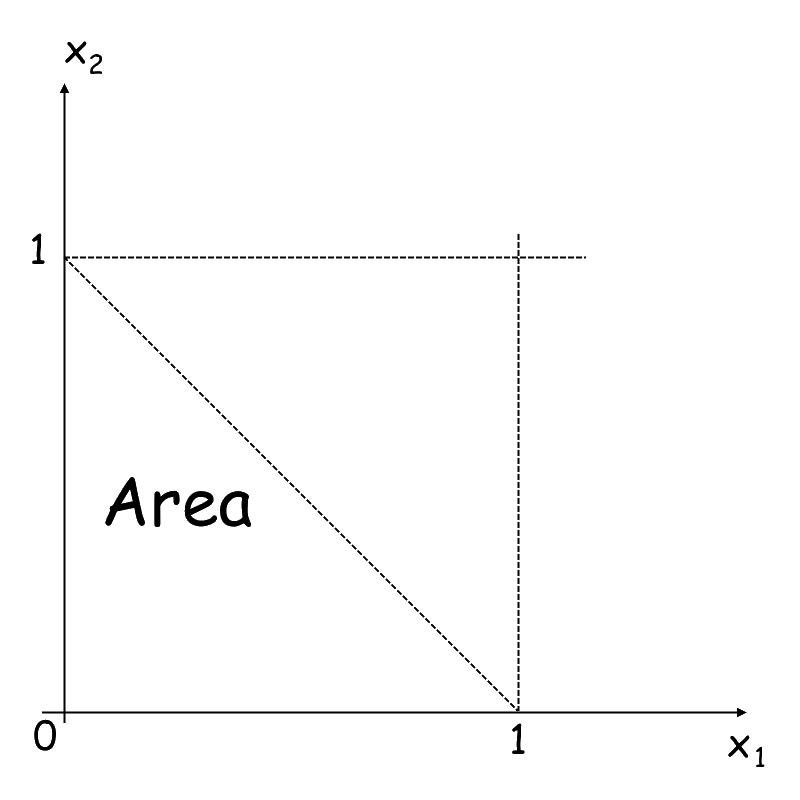
\includegraphics[scale=.5]{graph3.png}
				
				Therefore, $F_1(x_1)=2\mbox{``area"}=2(\frac{1}{2}(1)(1)-\frac{1}{2}(1-x_1)(1-x_1))=x_1(2-x_1)$ for all $x_1\in(0, 1)$. By symmetry, $F_2(x_2)=x_2(2-x_2)$ for all $x_2\in(0, 1)$.\\
				
				Thus, $F(\frac{1}{2}, \frac{1}{2})=\frac{1}{2}\neq\frac{9}{16}=F_1(\frac{1}{2})F_2(\frac{1}{2})$, so $X_1, X_2$ are not independent.\\
				
				Also note that $f(\underline{x})=2\neq2(1-x_1)2(1-x_2)=f_1(x_1)f_2(x_2)$ in general.
		\end{enumerate}
	\end{myex}
	
	\begin{myprop}{}{}
		For distribution functions $F_1, \dots, F_d$, there is a probability space $(\Omega, \mathcal{F}, P)$ and independent random variables $X_1, \dots, X_d$ such that $X_j\sim F_j$ for all $j\in\{1, \dots, d\}$.
		
		\begin{proof}
			Consider $\Omega=\R^d, \mathcal{F}=\mathcal{B}(\R^d), P(\prod_{j=1}^{d}B_j)=\prod_{j=i}^{d}P_{F_j}(B_j), X_j(\underline{\omega})=\omega_j$ for all $\underline{\omega}\in\R^d, j\in\{1, \dots, d\}$. Then, for all $j, X_j$ is measurable and
			
			\begin{align*}
				P(\bigcap_{j=1}^{d}X_j\inv(B_j))&=P(\bigcap_{j=1}^{d}\{\omega\in\Omega : X_j(\omega)\in B_j\})\\
				&=P(\prod_{j=1}^{d}B_j)\\
				&=\prod_{j=1}^{d}P(B_j)\\
				&=\prod_{j=1}^{d}P(X_j\inv(B_j))
			\end{align*}
			for all $B_1, \dots, B_d\in\mathcal{B}(\R)$ which implies $X_1, \dots, X_d$ are independent.\\
			
			Furthermore,
			\begin{align*}
				P(X_j\leq x_j)&=P(X_j\inv((-\infty, x_j]))\\
				&=\prod_{j=1}^{d}P_{F_j}(B_j)\\
				&=P_{F_j}((-\infty, x_j])\\
				&=F_j(x_j)
			\end{align*}
			So, $X_j\sim F_j$.
		\end{proof}
	\end{myprop}
	
	Infinite sequences of independent random variables $X_1, X_2, \dots$ can be constructed by involving ``Kolmogorov's extension theorem". In particular, can construct \ul{independent and identically distributed (iid)} random variables $X_1, X_2, \dots$ from a distribution function $F$ (universal df). In short, $X_1, X_2, \dots\sim F$.\\
	
	Interlude: Independence implies pairwise independence but not conversely.
	
	\begin{mydef}{}{}
		A \ul{copula} C is a distribution function with $U(0, 1)$ margins.
	\end{mydef}
	
	\begin{myprop}{}{}
		A function $C : [0, 1]^d\to[0, 1]$ is a $d$ dimensional copula iff:
		\begin{enumerate}[label=(\roman*)]
			\item $C(\underline{u})=0$ if $u_j=0$ for at least one $j\in\{1, \dots, d\}$. \textbf{(Groundedness)}
			
			\item $C(1, \dots, 1, u_j, 1, \dots, 1)=u_j$ for all $u_j\in[0, 1], j\in\{1, \dots, d\}$. \textbf{($U(0, 1)$ margins)}
			
			\item $\Delta_{(\underline{a}, \underline{b}]}C\geq0$ for all $(\underline{a}, \underline{b}])\in[0, 1]^d : \underline{a}\leq\underline{b}$. \textbf{(d-increasing)}
		\end{enumerate}
	\end{myprop}
	
	\begin{myex}{}{}
		\begin{enumerate}
			\item $C(\underline{u})=\prod(\underline{u}):=\prod_{j=1}^{d}u_j$ for $\underline{u}\in[0, 1]^d$ is a copula (independence copula). To show it's a density, show it's non-negative and differentiable.
			
			\item $C(\underline{u})=M(\underline{u})=\min\{u_1, \dots, u_d\}, \underline{u}\in[0, 1]^d$ is a copula (comonotone copula) since $\underline{U}\sim C$ for $\underline{U}=(U, \dots, U)$ with $U\sim U(0, 1)$.
			
			\begin{proof}
				\begin{align*}
					P(\underline{U}\leq\underline{u})&=P(U\leq u_1, \dots, U\leq u_d)\\
					&=P(U\leq\min\{u_1, \dots, u_d\})\\
					&=\min\{u_i, \dots, u_d\}\\
					&=C(\underline{u})
				\end{align*}
				for all $\underline{u}\in[0, 1]^d$.
			\end{proof}
			
			\item $C(\underline{u})=W(\underline{u}):=\max\{(\sum{j=1}^{d}u_j)-d+1, 0\}, \underline{u}\in[0, 1]^d$ is a copula (counter-monotone copula) iff $d=2$.
			
			\begin{proof}
				Suppose $d=2$. Let $\underline{U}=(U, 1-U)$ for $U\sim U(0, 1)$. Then
				\begin{align*}
					P(\underline{U}\leq\underline{u})&=P(\underline{U}\leq u_1, 1-U\leq u_2)\\
					&=P(1-u_2\leq U\leq u_1)\\
					&=\max\{u_1-(1-u_2), 0\}\\
					&=W(u_1, u_2)
				\end{align*}
				for all $u_1, u_2\in[0, 1]$.\\
				
				Suppose $d>2$. Then,
				\begin{align*}
					\Delta_{(\underline{\frac{1}{2}}, \underline{1}]}W=&\sum_{i\in\{0, 1\}^d}(-1)^{\sum_{j=1}^{d}i_j}W((\frac{1}{2})^{i_1}\cdot1^{1-i_1}, \dots, ((\frac{1}{2})^{i_d}\cdot1^{1-i_d})\\
					=&max\{1(d)-d+1, 0\}\\
					&-d\max\{1(d-1)+\frac{1}{2}-d+1, 0\}\\
					&+(2^d)\max\{1(d-2)+\frac{1}{2}+\frac{1}{2}-d+1, 0\}\\
					&-\dots+(-1)^d\max\{\frac{1}{2}(d)-d+1, 0\}\\
					=&1-\frac{d}{2}+0+\dots+0<0
				\end{align*}
				for $d>3$. Therefore, $W$ is not d-increasing (though it is componentwise increasing), so it is not a distribution.
			\end{proof}
		\end{enumerate}
	\end{myex}
	
	\begin{mythm}{Sklar's Theorem}{6.8}
		\begin{enumerate}
			\item For any distribution function $F$ with continuous margins $F_1, \dots, F_d$, there exists exactly one copula $C$: $$F(\underline{x})=C(F_1(x_2), \dots, F_d(x_d))$$ for all $\underline{x}\in\R^d$. (*) This copula is given by $$C(\underline{u})=F(F_1^-(u_1), \dots, F_d^-(u_d))$$ for all $u\in(0, 1)^d$.
			
			\item Given any copula $C$ and any univariate distribution functions $F_1, \dots, F_d$, $F$ defined by (*) is a distribution function with margins $F_1, \dots, F_d$.
		\end{enumerate}
		
		\begin{proof}~
			\begin{enumerate}
				\item Let $\underline{X}\sim F$ and $U:=(F_1(X_1), \dots, F_d(U_d))$. Then, $\underline{U}$ has $U(0, 1)$ margins, since
				\begin{align*}
					P(U_j\leq u_j)&=P(F_j(X_j)\leq u_j)\\
					&=P(F_j^-(F_j(X_j))\leq F_j^-(u_j))\\
					&=P(X_j\leq F^-(u_j))\\
					&=F_j(F_j^-(u_j))\\
					&=u_j
				\end{align*}
				for all $u_j\in(0, 1), j\in\{1, \dots, d\}$. So $U$ has a copula, say $C$, as its distribution function. Since
				\begin{align*}
					X_j&=F_j^-(F_j(X_j))\\
					&=F_j^-(u_j)
				\end{align*}
				for all $j$, therefore
				\begin{align*}
					F(\underline{x})&=P(X_j\leq x_j\;\forall j)\\
					&=P(F_j^-(u_j)\leq x_j\;\forall j)\\
					&=P(U_j\leq F_j(x_j)\;\forall j)\\
					&=C(F_1(x_1), \dots, F_d(x_d))
				\end{align*}
				for all $\underline{x}\in\R^d$, so $C$ satisfies (*). It is uniquely given by $C(u)=C(F_1(F_1^-(u_1)), \dots, F_d(F_d^-(u_d)))=F(F_1^-(u_1), \dots, F_d^-(u_d))$ for all $u\in(0, 1)^d$.
				
				\item Let $\underline{U}\sim C$, and $\underline{X}:=(F_1^-(U_1), \dots, F_d^-(U_d))$. Since
				\begin{align*}
					P(\underline{X}\leq\underline{x})=&=P(F_1^-(U_1)\leq x_1, \dots, F_d^-(U_d)\leq x_d)\\
					&=P(U_1\leq F_1(x_1), \dots, U_d\leq F_d(x_d))\\
					&=C(F_1(x_1), \dots, F_d(x_d))
				\end{align*}
				for all $x\in\R^d$, therefore $F$ defined by (*) is a distribution function, namely that of $\underline{X}$, with margins $F_1, \dots, F_d$ (by prop. \ref{pr:5.13}).
			\end{enumerate}
		\end{proof}
	\end{mythm}
	
	\begin{myrem}{}{}
		\begin{enumerate}
			\item Part (1) allows us to decompose any continuous $F$ into its copula and margins $F_1, \dots, F_d$. The copula is this precisely the function containing the information about the dependence between $X_1, \dots, X_d$ of $\underline{X}$.\\
			
			Part (2) allows us to construct flexible multivariate distribution functions.
			
			\item Two other important results:
			\begin{itemize}
				\item Fr\' ecbet-Hoeffding bounds: $W(\underline{u})\leq C(\underline{u})\leq M(\underline{u})$ for all $\underline{u}\in[0, 1]^d$ and copulas $C$.
				
				\item invariance principle: If $T_1, \dots, T_d$ are strictly increasing, then $(T_1(x_1), \dots, T_d(x_d))$ also has copula $C$.
			\end{itemize}
		\end{enumerate}
	\end{myrem}
	
	\section{Summary Statistics}
	In applications we often want to summarize a distribution function $F$ (or $X\sim F$) in terms of a real number, a summary statistic, such as
	\begin{itemize}
		\item $\alpha$-quantile $F^-(\alpha)$ (describes a location) is called the median of $F$ for $\alpha=\frac{1}{2}$.
		
		\item Mode of $F=\mbox{avg}\sup f(x)$ if $F$ has density $f$ or pmf $f$ (for the latter, the mode denotes the x-value most likely to appear).
		
		\item Mean of $F$ (describes the location of the average outcome or expected outcome), the variance (describes scale/variation/dispersion), if they exist.
	\end{itemize}
	
	\subsection{Expectation and moments}
	What value $\mu$ do you expect when rolling a fair die?\\
	
	Let $\Omega=\{1, \dots, 6\}, \mathcal{F}=\mathcal{P}(\Omega), P(A)=\frac{|A|}{|\Omega|}$ for $A\in\mathcal{F}$. Then, 
	\begin{align*}
		 \mu&=\sum_{\mbox{all outcomes}}\mbox{``outcome"}\cdot P(\mbox{``outcome"})\\
		 &=\sum_{\omega\in\Omega}\omega P(\{\omega\})\\
		 &=\sum_{i=1}^6i\cdot\frac{1}{6}\\
		 &=\frac{7}{2}
	\end{align*}
	Let $X(\omega)=\omega, X : \Omega\to\R$. Then, $\mu=\sum_{\omega\in\Omega}X(\omega)P(\{\omega\})$ is the mean or expectation of $X$ computed over $\Omega$. In the dice example, $P(X=x)=\frac{1}{6}$ for all $x\in S=\{1, \dots, 6\}$. We compute $\mu$ over $\R$ via
	\begin{align*}
		\mu&=\sum_{\omega\in S}xP(X=x)\\
		&=\sum_{\omega\in S}xf(x)
	\end{align*}
	If $X$ is absolutely continuous with density $f$, analogous formulas are
	\begin{align*}
		\mu&=\int_{\Omega}X(\omega)dP(\{\omega\})\\
		&=\int_{\Omega}xdP\mbox{ for shorthand}
		&=\int_{\R}xf(x)dx
	\end{align*}
	if these integrals exist, in which case one also writes $E(X)$ for $\mu$.\\
	
	Consider a general probability space $(\Omega, \mathcal{F}, P)$ with random variable $X$. In general, $E(X)$ can be constructed in 3 steps.
	
	\begin{enumerate}
		\item If $X=\sum_{i=1}^{n}x_i=\mathbbm{1}_{A_i}$ is simple, one can always define mean of $X$ as $$E(X):=\sum_{i=1}^{n}x_iP(A_i)=\sum_{i=1}^{n}x_iP(X=x_i)$$
		
		\item If $X\geq0$, mean of $X$ is defined by $$E(X):=\sup E(Y)$$ for simple $Y$ such that $0\leq Y\leq X$.
		
		\item In general, for $X=X^+-X^-$ where $X^+=\max\{X, 0\}$ and $X^-=-\min\{X, 0\}$, one defines $$E(X)=E(X^+)-E(X^-)$$ if $E(X^+)<\infty$ or $E(X^-)<\infty$. $E(X)$ is finite $\Leftrightarrow$ both $E(X^+)$ and $E(X^-)$ are finite $\Leftrightarrow$ $E(|X|)<\infty$ for $|X|=X^++X^-$.\\
		
		This process is known as algebraic induction and leads to this definition.
	\end{enumerate}
	
	\begin{mydef}{}{}
		Let $(\Omega, \mathcal{F}, P)$ be a probability space with random variable $X$. If $E(X^+)<\infty$ or $E(X^-)<\infty$, $X$ is \ul{quasi-integrable} and
		\begin{align*}
			E(X)&=\int_{\Omega}XdP\\
			&=\int_{\Omega}X(\omega)dP(\{\omega\})
		\end{align*}
		
		If $E(|X|)<\infty$ (notation: $X\in L^1(\Omega, \mathcal{F}, P)$), then $X$ is \ul{integrable} and $E(X)$ is the \ul{mean} or \ul{expectation} of $X$ (or its distribution or df).
	\end{mydef}
		
		We rarely compute expectations over $\Omega$, but rather over $\R$, in terms of df $F$ of $X$ (or its density/pmf). This is classified by this result (by algebraic induction).
		
		\begin{mythm}{Change of Variables}{7.2}
			Let $(\Omega, \mathcal{F}, P)$ be a probability space with random variable $X\sim F$. If $h : \R\to\R$ is measurable and $E(|h(X)|)<\infty$, then
			\begin{align*}
				\int_{\Omega}h(x)dP&=E(h(x))\mbox{ by definition}\\
				&=\int_{\R}h(x)dF(x)\mbox{ is the claim}\\
				&:=\begin{cases}
					\sum_{x\in S}h(x)f(x)&\mbox{ if $F$ is discrete, support is $S$, pmf is $f$}\\
					\int_{x\in\R}h(x)f(x)dx&\mbox{ if $F$ is abs. cont. with density $f$}
				\end{cases}
			\end{align*}
			(!!!)
		\end{mythm}
		
		\begin{myrem}{}{}
			\begin{enumerate}
				\item $E(|h(x)|)<\infty$ can be verified by showing $\int_{\R}|h(x)|dF(x)<\infty$. Often this is clear, such as if $h$ is bounded then
				\begin{align*}
					E(|h(x)|)&=\int_{\R}|h(x)|dF(x)\\
					&\leq M\int_{\R}dF(x)<\infty
				\end{align*}
				where $M$ is a real number.
				
				\item $E(h(x))$ can be computed over $\R$ via
				\begin{enumerate}[label=(\roman*)]
					\item $\int_{\R}h(x)dF_X(x)$ where $F_X$ is df of $X$; or by substitution via $h(x)=y$:
					
					\item $\int_{\R}ydF_y(y)$ where $F_y$ is df of $y=h(x)$.
				\end{enumerate}
				
				\item If $h(x)=x^p, p>0$, then p-th moment of $X\sim F$, if it exists, is $$E(x^p)=\int_{``\R"}x^pdF(x)$$
				One can use ``Holder's inequality" to show if $E(|x|^q)<\infty$ for some $q>p$, then $E(|x|^p)<\infty$ for all $0<p<q$. That is, higher moments existing imply lower moments existing.
				
				\item Proof of theorem \ref{th:7.2} readily extends to random vectors $\underline{X}\sim F$, measurable $\R^d\to\R$ such that $E(|h(x)|)<\infty$. In this case,
				\begin{align*}
					\int_{\Omega}h(\underline{x})dP&=E(h(\underline{X}))\\
					&=\int_{\R^d}h(\underline{x})dF(\underline{x})
				\end{align*}
				If $h(\underline{x})=x_1\cdot\dots\cdot x_d$, and $X_1, \dots, X_d$ are independent, then
				\begin{align*}
					E(X_1, \dots, X_d)&=\int_{\R^d}x_1\cdot\dots\cdot x_ddF(\underline{x})\\
					&=\int_{\R}\dots\int_{\R}x_1\dots x_ddF_1(x_1)\dots dF_d(x_d)\\
					&=\prod_{j=1}^{d}\int_{\R}x_jdF_j(x_j)\\
					&=E(x_1)\dots E(x_d)
				\end{align*}
			\end{enumerate}
		\end{myrem}
		
		\begin{myprop}{}{}
			Let $X, Y\in L^1(\Omega, \mathcal{F}, P)$. Then,
			\begin{enumerate}
				\item $aX+bY\in L^1(\Omega, \mathcal{F}, P)$ with $E(aX+bY)=aE(X)+bE(Y)$. \textbf{(linearity)}
				
				\item $A\in\mathcal{F}\Rightarrow E(\mathbbm{1}_A)=P(A)$
				
				\item $X\geq0$ almost surely $\Rightarrow E(X)\geq0$.
				
				\item $X\leq Y$ almost surely $\Rightarrow E(X)\leq E(Y)$.
				
				\item $X\geq0$ almost surely, $E(X)=0\Rightarrow X=0$ almost surely.
				
				\item $|E(X)|\leq E(|X|)$
				
				\item If $X\sim F$, then
				\begin{enumerate}[label=(\roman*)]
					\item $E(X)=\int_0^{\infty}\bar{F}(x)dx-\int_{-\infty}^0F(x)dx$ where $\bar{F}(x)=1-F(x)$.
					
					\item $E(x)=\int_0^1F^-(\alpha)d\alpha$
				\end{enumerate}
			\end{enumerate}
			
			\begin{proof}~
				\begin{enumerate}
					\item algebraic induction.
					
					\item $E(\mathbbm{1}_A)=1\cdot P(A)+0\cdot P(A_c)=P(A)$ since $\mathbbm{1}_A$ is simple
					
					\item $E(X)=E(X^+)\geq0$ since $X\geq0$ and by algebraic induction.
					\begin{enumerate}[label=(\roman*)]
						\item If $X$ is simple, $x_j\geq0\Rightarrow E(x)=\sum_{i=1}^nx_iP(A_i)\geq0$.
						
						\item Else, $\sup E(Y)\geq0$ over simple $Y$ such that $0\leq Y\leq X$.
					\end{enumerate}
					
					\item
					\begin{align*}
						E(Y)&=E(Y-X+X)\\
						&=E(Y-X)+E(X)\\
						&\geq E(X)
					\end{align*}
					since $Y-X\geq0$ almost surely, and thus $E(Y-X)\geq0$.
					
					\item Assume $P(X\geq0)$. Then,
					\begin{align*}
						\lim_{n\uparrow\infty}P(X>\frac{1}{n})&=\lim_{n\uparrow\infty}P(X\in(\frac{1}{n}, \infty])\\
						&=P(X\in\bigcup_{i=1}^{\infty}(\frac{1}{n}, \infty])\\
						&=P(X>0)\\
						&>0
					\end{align*}
					Therefore, there exists $n_0\in\N : P(X\geq\frac{1}{n})>0$ (*) for all $n\geq n_0$. For $\varepsilon=\frac{1}{n_0}>0$ (**), we have
					\begin{align*}
						0=E(X)&\geq E(X\cdot\mathbbm{1}_{\{X\geq\varepsilon\}})\\
						&\geq E(\varepsilon\mathbbm{1}_{\{X\geq\varepsilon\}})\\
						&=\varepsilon E(\mathbbm{1}_{\{X\geq\varepsilon\}})\\
						&=\varepsilon P(X\geq\varepsilon)\\
						&>0
					\end{align*}
					by (**) and (*).
					
					\item
					\begin{align*}
						|E(X)|&=|E(X^+)-E(X^-)|\\
						&\leq|E(X^+)+|E(X^-)|\\
						&=E(X^+)+E(X^-)\\
						&=E(X^++X^-)\\
						&=E(|X|)
					\end{align*}
					
					\item
					\begin{enumerate}[label=(\roman*)]
						\item Use integration by parts formula $$\int_a^bh(x)dF(x)=[h(x)F(x)]_a^b-\int_a^bF(x)dh(x)$$ and the fact that $$\int_{\R}h(x)dF(x)=-\int_{\R}h(x)d\bar{F}(x).$$
						We also need that
						\begin{enumerate}[label=(\alph*)]
							\item
							\begin{align*}
								0&\leq x\bar{F}(x)\\
								&=x(1-F(x))\\
								&=x(F(\infty)-F(x))\\
								&=x\int_{x}^{\infty}dF(z)\\
								&\geq\int_{x}^{\infty}zdF(z)\to0
							\end{align*}
							as $x\uparrow\infty$.
							
							\item $0\geq xF(x)=\int_{-\infty}^xxdF(z)\geq\int_{-\infty}^xzdF(z)\to0$ as $x\downarrow-\infty$, therefore,
							\begin{align*}
								E(X)&=\int_{\R}xdF(x)\\
								&=\int_0^{\infty}xdF(x)+\int_{-\infty}^0xdF(x)\\
								&=-\int_0^{\infty}xd\bar{F}(x)+\int_{-\infty}^0xdF(x)\\
								&=-([x\bar{F}(x)]_0^{\infty}-\int_0^{\infty}\bar{F}(x)dx)+[xF(x)]_{-\infty}^0-\int_{-\infty}^0F(x)dx
							\end{align*}
						\end{enumerate}
					\end{enumerate}
				\end{enumerate}
			\end{proof}
		\end{myprop}
		
		\begin{myprop}{}{}
			If $X$ is quasi-integrable, with $P(A)=0$, then $$\int_AXdP:=\int_{\Omega}X\mathbbm{1}_AdP=E(X\mathbbm{1}_A)=0$$
			
			\begin{proof}
				Let $X\geq0$. Then $X\mathbbm{1}_A\geq0$. Let $Y=\sum_{i=1}^{n}y_i\mathbbm{1}_{B_i}$ be simple, such that $0\leq Y\leq X\mathbbm{1}_A$ for all $\omega$. Then,
				\begin{align*}
					&0\leq y_i\mathbbm{1}_{B_i}\leq X\mathbbm{1}_A\mbox{ for }i=1, \dots, n\\
					\Rightarrow&y_i=0\mbox{ or }B_i\subseteq A\mbox{ for }i=1, \dots, n\\
					\Rightarrow&y_i=0\mbox{ or }P(B_i)\leq P(A)=0\\
					\Rightarrow&y_i=0\mbox{ or }P(B_i)=0\\
					\Rightarrow&E(Y)=\sum_{i=1}^{n}y_iP(B_i)\\
					\Rightarrow&E(X)=\sup_{0\leq Y\leq X, Y\mbox{ simple}}E(Y)=0
				\end{align*}
				for all $Y$. For general X, $$E(X\mathbbm{1}_A)=E(X^+\mathbbm{1}_A)-E(X^-\mathbbm{1}_A)=0$$
			\end{proof}
		\end{myprop}
		
		\subsection{Variance and Covariance}
		
		\begin{mydef}{}{}
			Let $(\Omega, \mathcal{F}, P)$ be a probability space with random variables $X, Y$ such that $E(X^2)<\infty, E(Y^2)<\infty$ (notation: $X, Y\in L^2(\Omega, \mathcal{F}, P)$). Then, $$\Var(X):=E((X-EX)^2)$$ is called the \ul{variance} of $X$ (or its distribution or df), and $\sqrt{\Var(X)}$ is the \ul{standard deviation}.\\
			
			The \ul{covariance} of $X, Y$ is defined by $$\Cov(X, Y):=E((X-EX)(Y-EY))$$ and the \ul{correlation} of $X, Y$ by $$\Cor(X, Y):=\frac{\Cov(X, Y)}{\sqrt{\Var(X)\Var(Y)}}$$
		\end{mydef}
		
		\begin{myrem}{}{7.7}
			Here are some properties of variance and covariance.
			\begin{enumerate}
				\item
				\begin{align*}
					\Var(X)&=E(X^2-2XE(X)+E(X)^2)\\
					&=E(X^2)-2E(X)E(X)+E(X)^2\\
					&=E(X^2)-E(X)^2
				\end{align*}
				Similarly,
				\begin{align*}
					\Cov(X, Y)&=E(XY)-E(X)E(Y)
				\end{align*}
				Also note that
				\begin{align*}
					\Cov(X, X)&=\Var(X)\\
					\Cov(X, c)&=0\;\forall c\in\R\\
					\Cov(X, Y)&=\Cov(Y, X)
				\end{align*}
				
				\item
				\begin{align*}
					\Var(X)=0&\Leftrightarrow E((X-EX)^2)=0\\
					&\Leftrightarrow(X-EX)^2=0\mbox{ almost surely}\\
					&\Leftrightarrow X-EX=0\mbox{ almost surely}\\
					&\Leftrightarrow X=EX\mbox{ almost surely}
				\end{align*}
				
				\item
				\begin{align*}
					\Var(aX+bY)&=E(((aX+bY)-E(aX+bY))^2)\\
					&=E((a(X-EX))^2)+2E(a(X-EX)b(Y-EY))+E((b(Y-EY))^2)\\
					&=a^2\Var(X)+2ab\Cov(X, Y)+B^2\Var(Y)
				\end{align*}
				for $a, b\in\R$. In particular if $Y=1$ almost surely, $\Var(aX+b)=a^2\Var(X)$.
				
				\item If $X, Y$ are independent, $$E(XY)=E(X)E(Y)$$ which implies $$\Cov(X, Y)=0=Cor(X, Y)$$
				So, independence implies uncorrelatedness. The converse is not true in general:\\
				
				Let $X\sim U(-1, 1), Y=X^2$. Then,\
				\begin{align*}
					\Cov(X, Y)&=E(XY)-E(X)E(Y)\\
					&=E(X^3)-0E(X^2)\\
					&=0
				\end{align*}
				by symmetry, since $X^3$ is an odd function. So $X, Y$ are uncorrelated but dependent.
			\end{enumerate}
		\end{myrem}
		
		\begin{myprop}{}{}
			Let $X, Y\in L^2(\Omega, \mathcal{F}, P)$. Then,
			\begin{align*}
				&\rho:=\Cor(X, Y)\in[-1, 1]\mbox{ and }|\rho|=1\\
				\Leftrightarrow&Y\mbox{ is a linear function of $X$ with slope }\lessgtr0\\
				\Leftrightarrow&\rho=\pm1
			\end{align*}
			
			\begin{proof}
				$(\Rightarrow)$ Let $z_t=tX+Y, t\in\R$. Let $a=t^2\Var(X), b=2t\Cov(X, Y), c=Var(Y)$. Then,
				\begin{align*}
					&0\leq\Var(z_t)=t^2\Var(X)+2t\Cov(X, Y)+Var(Y)\\
					\Rightarrow&0\geq b^2-4ac\\=(2\Cov(X, Y))^2-4\Var(X)\Var(Y)\\
					\Rightarrow&|\rho|=\sqrt{\rho^2}=\sqrt{\frac{\Cov(X, Y)^2}{\Var(X)\Var(Y)}}\leq1
				\end{align*}
				Furthermore, $|\rho|=1$ iff $b^2-4ac=0$
				\begin{align*}
					\Rightarrow&\exists!\tilde{t}\in\R: \Var(z_{\tilde{t}})=0\\
					\Rightarrow&\tilde{t}X+Y=c\in\R\mbox{ almost surely}\\
					\Rightarrow&Y=c-\tilde{t}X\mbox{ almost surely}\\
				\end{align*}
				In this case,
				\begin{align*}
					\rho&=\frac{\Cov(X, c-\tilde{t}X}{\sqrt{\Var(X)Var(c-\tilde{t}X}}\\
					&=\frac{-\tilde{t}\Cov(X, X)}{\sqrt{\Var(X)\tilde{t}^2\Var(X)}}\\
					&=\frac{\tilde{t}\Var(X)}{|\tilde{t}|\Var(X)}\\
					&=\frac{-\tilde{t}}{|\tilde{t}|}
				\end{align*}
				So, $-\tilde{t}\lessgtr0$ iff $\rho=\pm1$. $(\Leftarrow)$ is trivial.
			\end{proof}
		\end{myprop}
		
		\section{Examples of Distributions}
		\subsection{Discrete Distributions}
		\subsubsection{Discrete Uniform Distribution}
		\begin{itemize}
			\item Notation:$U(\{x_1, \dots, x_n\})$
			\item $X\sim U(\{x_1, \dots, x_n\})$ models n distinct outcomes, each with equal probability $\frac{1}{n}$.
			\item PMF: \[f(x)=
						\begin{cases}
							\frac{1}{n}&x\in\{x_1, \dots, x_n\}\\
							0&\mbox{otherwise}
						\end{cases}\]
			Check: $f(x)\geq0$ for $x\in\R$, and $\sum_{i=1}^{n}f(x_n)=\frac{1}{n}n=1$
			
			\item Distribution function:
			\begin{align*}
				F(x)&=P(X\leq x)\\
				&=\sum_{k\in\{1, \dots, n\} : x_k\leq x}P(X=x_k)\\
				&=\frac{1}{n}|\{x_k : x_k\leq x\}|
			\end{align*}
			If $x_k=k$, we have
			\begin{align*}
				F(x)&=\begin{cases}
					0&x<1\\
					\frac{\lfloor x\rfloor}{n}&x\in[1, n)\\
					1&x\geq n
				\end{cases}
			\end{align*}
			\item Mean: We have $E(X)=\sum_{k=1}^{n}x_kP(X=x_k)=\frac{1}{n}\sum_{k=1}^{n}x_k$. If $x_k=k$, then $E(X)=\frac{n+1}{2}$.
			\item Variance: We have $\Var(X)=E(X^2)-E(X)^2=\frac{1}{n}\sum_{k=1}^{n}x_k^2-(\frac{1}{n}\sum_{k=1}^{n}x_k)^2$. If $x_k=k$, then $\Var(X)=\frac{1}{n}\frac{n(n+1)(2n+1)}{6}-(\frac{n+1}{2})^2=\frac{n^2-1}{12}$.
			\begin{myrem*}{}{}
				If $U\sim U(0, 1)$, then $\lceil nU\rceil\sim U(\{1, \dots, n\})$ since
				\begin{align*}
					P(nU=k)&=P(k-1<nU\leq k)\\
					&=P(U\in(\frac{k-1}{n}, \frac{k}{n}])\\
					&=\frac{k}{n}-\frac{k-1}{n}\\
					&=\frac{1}{n}
				\end{align*}
				for $k=1, \dots, n$. In particular, $X=x_{\lceil nU\rceil}\sim U(\{1, \dots, n\})$
			\end{myrem*}
		\end{itemize}
		
		\subsubsection{Binomial Distribution}
		\begin{itemize}
			\item Notation: $B(n, p)$ where $n\geq1, p\in(0, 1)$.
			\item $X\sim B(n, p)$ models the number of successes when independently repeating same experiment with outcomes success or failure $n$ times, where $P(\mbox{success})=p$. These experiments are \ul{Bernoulli trials}. Then, $X=\sum_{k=1}^{n}X_k$ for $X_1, \dots, X_n\sim B(1, p)$.
			\item PMF: \[f(x)=
						\begin{cases}
							\binom{n}{x}p^x(1-p)^{n-x}&x\in\{0, \dots, n\}\\
							0&\mbox{otherwise}
						\end{cases}\]
			Check: $f(x)\geq0$ for $x\in\R$, and
			\begin{align*}
				\sum_{k=0}^{n}\binom{n}{x}p^k(1-p)^{k}&=(p+(1-p))^n\\
				&=1
			\end{align*}
			\item Distribution function:
			\begin{align*}
				F(X)&=P(X\leq x)\\
				&=P(X\leq\lfloor x\rfloor)\\
				&=\sum_{k=0}^{\lfloor x\rfloor}\binom{n}{x}p^k(1-p)^{n-k}\\
				&=\int_{p}^{1}f_{x, n}(z)dz
			\end{align*}
			where $f_{x, n}$ is the density of the Beta($x+1, n-x$) distribution. By letting $p=0$, this gives 1 for $x\in[0, n]$.
			\item Mean:
			\begin{align*}
				E(X)&=\sum_{k=1}^{n}k\binom{n}{k}p^k(1-p)^{n-k}\\
				&=np\sum_{k=1}^{n}\frac{(n-1)!}{(k-1)!(n-k)!}p^{k-1}(1-p)^{n-k}\\
				&=np\sum_{k=0}^{n-1}\binom{n-1}{k}p^k(1-p)^{n-k}\\
				&=np
			\end{align*}
			From knowing the PMF of the Beta distribution. Or,
			\begin{align*}
				E(X)&=E(\sum_{k=1}^{n}X_k)\\
				&=\sum_{k=1}^{n}E(X_k)\\
				&=np
			\end{align*}
			\item Variance:
			\begin{align*}
				E(X^2)-E(X)&=E(X(X-1))\\
				&=\sum_{k=2}^{n}k(k-1)\frac{n!}{k!(n-k)!}p^k(1-p)^{n-k}\\
				&=p^2n(n-1)\sum_{k=2}^{n}\binom{n-2}{k-2}p^{k-2}(1-p)^{n-k}\\
				&=p^2n(n-1)\\
				\Rightarrow E(X^2)&=p^2n(n-1)+np\\
				\Var(X)&=p^2n(n-1)+np-(np)^2\\
				&=np(1-p)
			\end{align*}
			Or,
			\begin{align*}
				\Var(X)&=\Var(\sum_{k=1}^{n}X_k)\\
				&=\sum_{k=1}^{n}Var(X_k)+2\sum_{1\leq k\leq l\leq n}\Cov(X_k, X_l)\\
				&=np(1-p)
			\end{align*}
			since $\Var(X_k)=E(X_k^2)-E(X_k)^2=p-p^2$
			\begin{myrem*}{}{}
				If you participate in weekly lottery, with 2\% probability of winning each week, then the number of wins in one year is $B(52, 0.02)$ distributed.
			\end{myrem*}
		\end{itemize}
		
		\subsubsection{Geometric Distribution}
		\begin{itemize}
			\item Notation: $Geo(p), p\in(0, 1)$
			\item $X\sim Geo(p)$ models the number of independent Bernoulli trials with success probability $p$ until first success.
			\item PMF: \[f(x)=\begin{cases}
							p(1-p)^{x-1}&x\in\N\\
							0&\mbox{otherwise}
						\end{cases}\]
			Check: $f(x)\geq0$ for $x\in\R$. $\sum_{k=1}^{\infty}p(1-p)^{k-1}=p\sum_{k=0}^{\infty}(1-p)^{k-1}=p\frac{1}{1-(1-p)}=1$
			\item Distribution function:
					\begin{align*}
						F(x)&=P(X\leq\lfloor x\rfloor)\\
						&=\sum_{k=1}^{\lfloor x\rfloor}p(1-p)^{k-1}\\
						&=p\sum_{k=0}^{\lfloor x-1\rfloor}p(1-p)^{k-1+1}\\
						&=p\frac{1-(1-p)^{\lfloor x\rfloor}}{1-(1-p)}\\
						&=1-(1-p)^{\lfloor x\rfloor}
					\end{align*}
					for $x\in[1, \infty)$.
			\item Mean: Note that
					\begin{align*}
						\sum_{k=1}^{\infty}kq^{k-1}&=\frac{d}{dq}\sum_{k=1}^{\infty}q^k\\
						&=\frac{d}{dq}(\frac{1}{1-q}-1)\\
						&=\frac{1}{(1-q)^2}
					\end{align*}
					for $|q|<1$. Therefore,
					\begin{align*}
						E(X)&=\sum_{k=1}^{\infty}kp(1-p)^{k-1}\\
						p\frac{1}{1-(1-p)^2}\\
						&=\frac{1}{p}
					\end{align*}
			\item Variance: Note that
					\begin{align*}
						\sum_{k=2}^{\infty}k(k-1)q^{k-2}&=\sum_{k=0}^{\infty}\frac{d^2}{dq^2}q^k\\
						&=\frac{d^2}{dq^2}(\frac{1}{1-q}-q-1)\\
						&=\frac{2}{(1-q)^3}
					\end{align*}
					for $|q|<1$. Therefore,
					\begin{align*}
						E(X(X-1))&=\sum_{k=2}^{\infty}k(k-1)p(1-p)^{k-1}\\
						&=p(1-p)\sum_{k=2}^{\infty}k(k-1)(1-p)^{k-2}\\
						&=p(1-p)(\frac{2}{(1-(1-p))^3}\\
						&=\frac{2(1-p)}{p^2}\\
						\therefore E(X^2)&=\frac{2(1-p)}{p^2}+E(X)=\frac{2-p}{p^2}\\
						\therefore\Var(X)&=\frac{1-p}{p^2}
					\end{align*}
					\begin{myrem*}{}{}
						\begin{enumerate}
							\item How many weeks to play the lottery such that probability of first win is at least 95\%? If $X\sim Geo(0.02)$, we need to find smallest $n$ such that
							\begin{align*}
								P(X\leq n)\geq0.95&\Leftrightarrow1-(1-0.02)^n\geq0.95\\
								&\Leftrightarrow0.5\geq0.98^n\\
								&\Leftrightarrow n\geq\lceil\frac{\log(0.05)}{\log(0.98)}\rceil=149
							\end{align*}
							
							\item As in R, geometric distribution is sometimes defined on $\N_0$. If $X\sim Geo(p)$, $Y:=X-1$ has PMF $f_Y(x)=p(1-p)^x$, expectation $E(Y)=\frac{1}{p}-1=\frac{1-p}{p}$, variance $\Var(Y)=Var(X)$. Here, $Y$ is interpreted as the number of failures before a success.
						\end{enumerate}
					\end{myrem*}
				\end{itemize}
				
		\subsubsection{Poisson Distribution}
		\begin{itemize}
			\item Notation: $Poi(\lambda), \lambda>0$
			\item $X\sim Poi(\lambda)$ models the number of events occurring in fixed time interval, if these events occur at fixed rate $\lambda$ and independently of time of last event.
			\item PMF: \[f(x)=\begin{cases}
								\frac{\lambda^x}{x!}e^{-\lambda}&x\in\N_0\\
								0&\mbox{ otherwise}
								\end{cases}\]
			Check: $f(x)\geq0$ for $x\in\R$. $\sum_{x=0}^{\infty}f(x)=\sum_{k=0}^{\infty}\frac{\lambda^k}{k!}e^{-\lambda}=e^{\lambda}e^{-\lambda}=1$
			\item Distribution function:
					\begin{align*}
						F(x)&=\sum_{k=0}^{\lfloor x\rfloor}\frac{\lambda^k}{k!}e^{-\lambda}
					\end{align*}
					for $x\in\R$. R uses $F(x)=\frac{\Gamma(\lfloor x\rfloor+1, \lambda)}{\lfloor x\rfloor!}$, where $\Gamma(s, z)=\int_{z}^{\infty}t^{s-1}e^{-t}dt$ is the upper incomplete gamma function.
			\item Mean:
					\begin{align*}
						E(X)&=\sum_{k=1}^{\infty}k\frac{\lambda^k}{k!}e^{-\lambda}\\
						&=\lambda\sum_{k=1}^{\infty}\frac{\lambda^{k-1}}{(k-1)!}e^{-\lambda}\\
						&=\lambda
					\end{align*}
			\item Variance:
					\begin{align*}
						E(X(X-1))&=\sum_{k=2}^{\infty}k(k-1)\frac{\lambda^k}{k!}e^{-\lambda}\\
						&=\lambda^2\sum_{k=2}^{\infty}\frac{\lambda^{k-2}}{(k-2)!}e^{-\lambda}\\
						&=\lambda^2\\
						\Rightarrow E(X^2)&=\lambda^2+\lambda\\
						\Rightarrow\Var(X)&=\lambda^2+\lambda-\lambda^2=\lambda
					\end{align*}
					\begin{myrem*}{}{}
						\begin{enumerate}
							\item What is probability of obtaining more than 12 emails per hour if you receive 240 emails per day on average?
							\begin{align*}
								\lambda&=E(X)\\
								&=\frac{240}{24}\\
								&=10
								\Rightarrow P(X>12)&=\sum_{k=13}^{\infty}\frac{10^k}{k!}e^{-10}\\
								&\approx22.84\%
							\end{align*}
							In R, this can be calculated using \begin{verbatim}
								ppois(12, lambda=10, lower.tail=FALSE)
							\end{verbatim}
							
							\item Suppose we divide the time interval in (1) into $n$ equal parts, and assume one only receives 0 or 1 emails in each of the $n$ intervals (1 email with probability $p$). Then for $n\to\infty, p\downarrow0$ such that $np\to\lambda$, we obtain
							\begin{align*}
								P(X=x)&=\binom{n}{x}p^x(1-p)^{n-x}\\
								&=\frac{n(n-1)\dots(n-x+1)}{n^x}\frac{(np)^x}{x!}(1-\frac{np}{n})(1-p)^{-x}
							\end{align*}
							(***) Which is the $Poi(\lambda)$ distribution as the limit of the $B(n, p)$ distribution. Note: if $a_n\to a$ as $n\to\infty$, $(1+\frac{a_n}{n})^n\to e^a$ as $n\to\infty$.
						\end{enumerate}
					\end{myrem*}
				\end{itemize}
		
		\subsection{Absolutely Continuous Distributions}
		\subsubsection{Continuous Uniform Distribution}
		\begin{itemize}
			\item Notation: $U(a, b)$ for $a, b\in\R, a<b$.
			\item $X\sim U(a, b)$ models outcomes uniformly distributed over $(a, b)$, that is, $P(X\in(x, x+h])$ is constant and equals $\frac{h}{b-a}$ for all $x\in[a, b-h]$. See Example \ref{ex:5.17} (1).
			\item Density: \[f(x)=\frac{1}{b-a}\mathbbm{1}_{(a, b]}(x)\] for $x\in\R$.
			Check: $f(x)\geq0$ for $x\in\R$. Also, $\int_a^b\frac{1}{b-a}dz=\frac{1}{b-a}\int_a^b(1)dz=\frac{b-a}{b-a}=1$.
			\item Distribution function:
					\begin{align*}
						F(x)&=P(X\leq x)\\
						&=\int_{-\infty}^xf(z)dz\\
						&=\int_a^x\frac{1}{b-a}dz\\
						&=\frac{x-a}{b-a}
					\end{align*}
					for $x\in[a, b]$.
			\item Moments:
					\begin{align*}
						E(X^k)&=\int_a^bx^kf(x)dx\\
						&=\frac{1}{b-a}\int_a^bx^kdx\\
						&=\frac{b^{k+1}-a^{k+1}}{(b-a)(k+1)}\\
						&=\frac{\sum_{l=0}^{k}a^lb^{k-l}}{k+1}\\
						\Rightarrow E(X)&=\frac{b-a}{2}\\
						\Var(X)&=E(X^2)-E(X)^2\\
						&=\frac{(b-a)^2}{12}
					\end{align*}
			\begin{myrem*}{}{}
				\begin{enumerate}
					\item $U(0, 1)$ is the standard uniform distribution.
					
					\item It is an important building block for other distributions. For example, it is used in
					\begin{itemize}
						\item Inversion method ($F^-(U)\sim F$)
						\item Sklar's Theorem (where we used $F(X)\sim U(0, 1)$ if $F$ is continuous and $X\sim F$)
						\item Sampling from $U(\{1, \dots, n\})$
					\end{itemize}
					
					\item $U\sim U(0, 1)\Rightarrow X : a+(b-a)U\sim U(a, b)$ is the stochastic representation of $U(a, b)$. (***)
				\end{enumerate}
			\end{myrem*}
		\end{itemize}
		
		\subsubsection{Gamma Distribution}
		\begin{itemize}
					\item Notation: $\Gamma(\alpha, \beta)$ where $\alpha>0$ is the shape, $\beta>0$ is the rate.
					\item Special cases:
					\begin{itemize}
						\item Exponential distribution
						\item Erlang distribution
						\item Chi-squared distribution
					\end{itemize}
					\item Density: \[f(x)=\frac{\beta^x}{\Gamma(x)}x^{\alpha-1}e^{-\beta x}\] for $x>0$ where $$\Gamma(x)=\int_0^{\infty}t^{\alpha-1}e^{-\infty}dt$$ is the gamma function.
					Check: $f(x)\geq0$ for $x\in\R$. Also,
					\begin{align*}
						\int_0^{\infty}\frac{\beta^{\alpha}}{\Gamma(x)}z^{\alpha-1}e^{-\beta z}dz&=\frac{1}{\Gamma(x)}\int_0^{\infty}\beta^{\alpha}(\frac{t}{\beta})^{\alpha-1}e^{-t}\frac{1}{\beta}dt\mbox{ Let $t=\beta z$}\\
						&=\frac{1}{\Gamma(x)}\Gamma(x)\\
						&=1
					\end{align*}
					\item Distribution function:
							\begin{align*}
								F(x)&=\int_0^x\frac{\beta^{\alpha}}{\Gamma(\alpha)}e^{-\beta z}z^{\alpha-1}dz\\
								&=\frac{1}{\Gamma(x)}\int_0^{\beta x}t^{\alpha-1}e^{-t}dt\mbox{ Let $t=\beta z$}\\
								&=\frac{\gamma(\alpha, \beta x)}{\Gamma(\alpha)}
							\end{align*}
							where $\gamma$ is the lower incomplete gamma function (available numerically).
					\item Moments:
							\begin{align*}
								E(X^k)&=\frac{\beta^{\alpha}}{\Gamma(x)}\int_0^{\infty}x^{k-\alpha-1}e^{-\beta x}dx\\
								&=\frac{\beta^{\alpha}}{\Gamma(\alpha)}\frac{k(k+\alpha)}{\beta^{k+\alpha}}\int_0^{\infty}\frac{\beta^{k+\alpha}}{\Gamma(k+\alpha}x^{k+\alpha-1}e^{-\beta x}dx\\
								&=\frac{\beta^{-k}\Gamma(k+\alpha)}{\Gamma(\alpha)}\\
								&=\beta^{-k}\frac{(k_\alpha-1)\cdot\dots\cdot(\alpha\Gamma(\alpha))}{\Gamma(\alpha)}\\
								&=\beta^{-k}\prod_{i=0}^{k-1}(i+\alpha)\\
								\Rightarrow E(X)&=\frac{\alpha}{\beta}\\
								\Var(X)&=E(X^2)-E(X)^2\\
								&=\frac{\alpha(1+\alpha)}{\beta^2}-(\frac{\alpha}{\beta})^2\\
								&=\frac{\alpha}{\beta}
							\end{align*}
					\begin{myrem*}{}{}
						\begin{enumerate}
							\item $Y\sim\Gamma(\alpha, 1)\Rightarrow X=\frac{Y}{\beta}\sim\Gamma(\alpha, \beta)$ since
							\begin{align*}
								F_X(x)&=P(X\leq x)\\
								&=P(\frac{Y}{\beta}\leq x)\\
								&=P(Y\leq\beta x)\\
								&=F_Y(x)\\
								&=\int_0^{\beta x}\frac{1}{\Gamma(x)}t^{\alpha-1}e^{-t}dt\mbox{ Let $t=\beta z$}\\
								&=\int_0^x\frac{\beta^{\alpha}}{\Gamma(x)}z^{\alpha-1}e^{-\beta z}dz
							\end{align*}
							
							\item Parametrization: $f(x)=\frac{1}{\Gamma(x)s^{\alpha}}x^{\alpha-1}e^{-\frac{x}{s}}$ for $s>0$ is also used frequently. See also R's
							\begin{verbatim}
								dgamma(x, shape, rate=1, scale=1/rate)
							\end{verbatim}
						\end{enumerate}
					\end{myrem*}
				\end{itemize}
				
			\subsubsection{Exponential Distribution}
			\begin{itemize}
				\item Notation: $Exp(\lambda)$, $\lambda>0$ (rate)
				\item $X\sim Exp(\lambda)$ describes interarrival times between events in a (homogeneous) Poisson (point) process with intensity $\lambda>0$, that is, a sequence of random variables $(\N_t)_{t\geq0}$ such that:
				\begin{enumerate}[label=(\roman*)]
					\item $N_0=0$
					\item $\forall n\in\N$ and $0\leq t_0<\dots<t_n<\infty$, the increments $N_{t_1}-N_{t_0}, \dots, N_{t_n}-N_{t_{n-1}}$ are independent
					\item $N_t-N_s\sim Poi(\lambda(t-s))$ for $0\leq s<t$ for some $\lambda>0$.
				\end{enumerate}
				Such continuous-time stochastic processes model the numebr of events in a process in which events occur continuously, independently at a constant rate $\lambda>0$ per unit (here, time) interval. Note that $N_t-N_s=N_{ts}-N_0=N_{ts}$ for $0\leq s<t$.
				\item Density: \[f(x)=\lambda e^{-\lambda x}\] for $x\geq0$.
				Check: $f(x)\geq0$ for $x\in\R$. Also, $\int_0^{\infty}\lambda e^{-\lambda x}dx=1$. Note that $f(x)$ is $\Gamma(1, x)$ density, so $Exp(\lambda)=\Gamma(1, \lambda)$.
				\item Distribution function:
						\begin{align*}
							F(x)&=\int_0^x\lambda e^{-\lambda z}dz=1-e^{\lambda x}
						\end{align*}
						for $x\geq0$.
				\item Moments:
						\begin{align*}
							E(X^k)&=\lambda^{-k}\prod_{i=0}^{k-1}(i+1)\\
							&=\frac{k!}{\lambda^k}\\
							\Rightarrow E(X)&=\frac{1}{\lambda}\\
							\Var(X)&=\frac{2}{\lambda^2}-(\frac{1}{\lambda})^2=\frac{1}{\lambda^2}
						\end{align*}
				\begin{myrem*}{}{}
					\begin{enumerate}
						\item $U\sim U(0, 1)\Rightarrow X=\frac{-1}{\lambda}\log(U)\sim Exp(\lambda)$ is the stochastic representation.
						
						\item $X\sim Exp(\lambda)\Rightarrow Y=\lceil X\rceil\sim Geo(1-e^{-\lambda})$ since
						\begin{align*}
							f_Y(k)&=P(\lceil X\rceil=k)\\
							&=P(X\in(k-1, k])\\
							&=F_X(k)-F_X(k-1)\\
							&=1-e^{-\lambda k}-(1-e^{-\lambda(k-1)})\\
							&=(e^{-\lambda})^{k-1}(1-e^{-\lambda})
						\end{align*}
						for $k\in\N$.
						
						\item $Exp(\lambda)$ is the only continuous memoryless distribution in the sense that $X\sim Exp(\lambda)$ satisfies $$P(X>s+t | X>s)=P(X>t)$$ for $s, t\geq0$. Similarly, $Geo(p)$ is the only discrete memoryless distribution.
						
						\item If $(N_t)_{t\geq0}$ is a Poisson process with intensity $\lambda>0$, let $$T_k:=\min\{t\geq0 : N_t=k\}$$ denote arrival time of k-th event, $k\in\N_0$. Then,
						\begin{align*}
							P(\mbox{``interarrival time between k-th and (k+1)-th event is $>x$"})\\
							&=P(T_{k+1}-T_{k}>x)\\
							&=P(N_{T_{k+x}}=k)\\
							&=P(N_{T_{k}+x}=N_{T_k})\\
							&=P(N_{T_{k}+x}-N_{T_k}=0)\\
							&=P(N_x=0)\\
							&=\frac{(\lambda x)^0}{0!}e^{-\lambda x}\\
							&=e^{-\lambda x}\\
							\Rightarrow T_{k+1}-T_k&\sim Exp(\lambda)
						\end{align*}
						for $k\in\N_0$. So, interarrival times in a Poisson process with intensity $\lambda>0$ are $Exp(\lambda)$ distributed from this stochastic process.
						
						\item For a sequence $(Y_k)_{k\in\N}$ of non-negative random variables, the \ul{compound Poisson process} $$X_t=\sum_{k=1}^{N_t}Y_k$$ is an important stochastic process in applications.
					\end{enumerate}
				\end{myrem*}
			\end{itemize}
			
			\subsubsection{Normal Distribution}
			\begin{itemize}
						\item Notation: $N(\mu, \sigma^2)$ where $\mu\in\R$ is the mean/location, and $\sigma>0$ is the standard deviation/scale.
						\item $X\sim N(\mu, \sigma^2)$ models outcomes which fluctuate symmetrically around $\mu$ with variance $\sigma^2$.
						\item Density: \[f(x)=\frac{1}{\sqrt{2\pi\sigma^2}}e^{\frac{-1}{2}(\frac{x-\mu}{\sigma})^2}\] for $x\in\R$.
						Check: See example \ref{ex:5.17} (2).
						\item Distribution function: Only available numerically.
						\item Mean:
						\begin{align*}
							E(X)&=\mu
						\end{align*}
						by calculus.
						\item Variance:
						\begin{align*}
							\Var(X)&=\sigma^2
						\end{align*}
						by calculus.
						\begin{myrem*}{}{}
							\begin{enumerate}
								\item $N(0, 1)$ is known as the standard normal distribution, and its df and density are denoted by $\Phi$ and $\phi$ respectively.
								
								\item $Z\sim N(0, 1)\Leftrightarrow X:=\mu+\sigma Z\sim N(\mu, \sigma^2)$ since
								\begin{align*}
									F_X(x)&=P(X\leq x)\\
									&=P(\mu+\sigma Z\leq x)\\
									&=P(z\leq\frac{x-\mu}{\sigma})\\
									&=\Phi(\frac{x-\mu}{\sigma})
								\end{align*}
								for $x\in\R$
								\begin{align*}
									\Leftrightarrow f_X(x)&=\phi(\frac{x-\mu}{\sigma})\frac{1}{\sigma}\\
									&=\frac{1}{\sqrt{2\pi\sigma^2}}e^{\frac{-1}{2}(\frac{x-\mu}{\sigma})^2}
								\end{align*}
								which is the density of $N(\mu, \sigma^2)$. Since $E(Z)=0$, $\Var(Z)=1$, we obtain $E(X)=\mu+\sigma Z$ and $\Var(X)=\sigma^2\Var(Z)=\sigma^2$
								
								\item Sketch of $f$ (bell curve):\\
								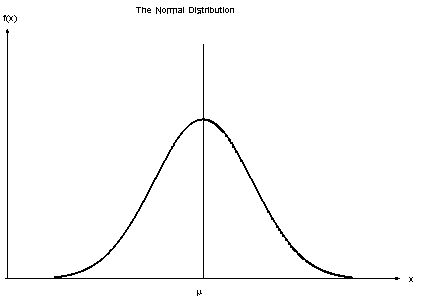
\includegraphics[scale=1]{normal.png}
								
								Since $f(\mu+x)=f(\mu-x)$ for $x\in\R$,
								\begin{align*}
									F(\mu-x)&=1-F(\mu+x)
								\end{align*}
								for $x\in\R$ by calculus. We can sketch $F(x)$:\\
								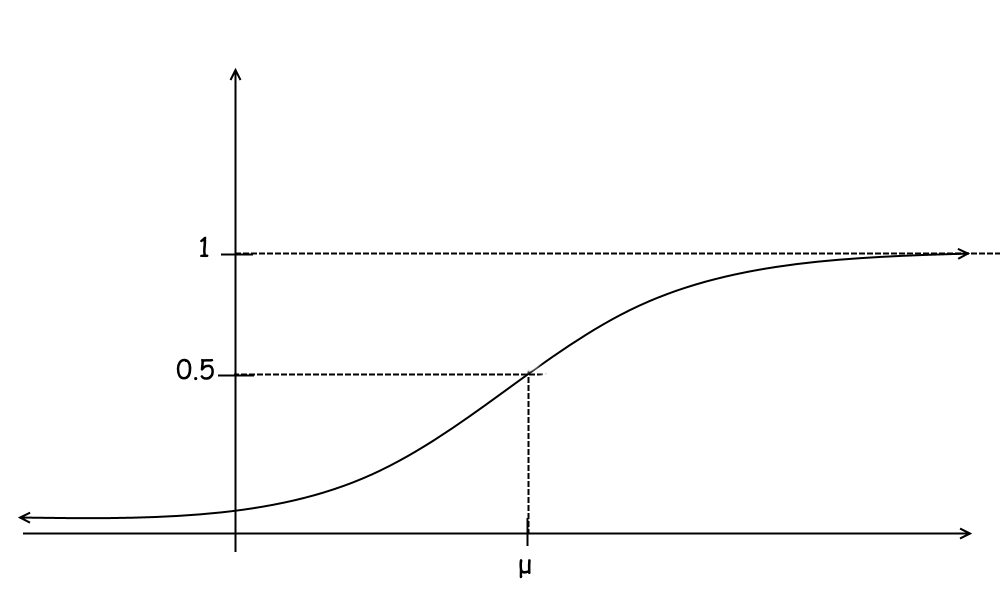
\includegraphics[scale=.5]{normaldist.png}
								
								Therefore to evaluate distribution function of $F$ of $N(\mu, \sigma^2)$ it suffices to know $\Phi(x)$ for all $x\in\R$.
							\end{enumerate}
						\end{myrem*}
					\end{itemize}
					
			\newpage
			\subsection{Multivariate Distributions}
			\subsubsection{Mean vector, Covariance and Correlation Matrices}
			
			\begin{mydef}{}{}
				Let $\underline{X}=(X_1, \dots, X_d)$. If $E(|X_j|)\leq\infty$ for all j, the \ul{mean vector} or expectation of $\underline{X}$(or its distribution function or distribution) is defined $$\underline{\mu}=E(\underline{X})=(E(X_1), \dots, E(X_d))$$
				
				If $E(X_j)<\infty$ for all j, the \ul{covariance and correlation matrices} is defined by
				\begin{align*}
					\Sigma&=\Cov(\underline{X})=(\Cov(X_i, X_j))_{i, j=1, \dots, d}\\
					P&=\Cor(\underline{X})=(\Cor(X_i, X_j))_{i, j=1, \dots, d}
				\end{align*}
			\end{mydef}
			
			\begin{mylem}{}{}
				\begin{enumerate}
					\item $E(A\underline{X}+\underline{b})=AE(\underline{X})+\underline{b}$. In particular, $E(\underline{a^T}\,\underline{X})=\underline{a^T}E(\underline{X})$.
					
					\item $\Cov(A\underline{X}+\underline{b})=A\Cov(\underline{X})A^T$. In particular, $\Var(\underline{a^T}\,\underline{X})=\Cor(\underline{a^T}\,\underline{X})=\underline{a^T}\Cov(X)\underline{a}$.
				\end{enumerate}
				\begin{proof}
					\begin{enumerate}
						\item
						\begin{align*}
							(E(A\underline{x}+\underline{b}))_j&=E(\sum_{k=1}^{d}a_{jk}X_k+b_j)\\
							&=\sum_{k=1}^{d}a_{jk}E(X_k)+b_j\\
							&=(AE(X)+b)_j
						\end{align*}
						for all j.
						
						\item
						\begin{align*}
							\Cov(A\underline{X}+\underline{b})_{ij}&=\Cov((A\underline{X}+\underline{b})_i, (A\underline{X}+\underline{b})_j)\\
							&\Cov(\sum_{k=1}^da_{ik}X_k+b_i, \sum_{l=1}^da_{jl}X_l+b_j)\\
							&=E((\sum_{k=1}^{d}a_{ik}(X_k-E(X_k)))(\sum_{l=1}^{d}a_{jl}(X_l-E(X_l))))\\
							&=E(\sum_{k=1}^{d}\sum_{l=1}^{d}a_{ik}a_{jl}(X_k-E(X_k))(X_l-E(X_l)))\\
							&=\sum_{k=1}^{d}\sum_{l=1}^{d}a_{ik}a_{jl}\Cov(X_k, X_l)\\
							&=A\Cov(\underline{X})A^T
						\end{align*}
						In particular,
						\begin{align*}
							\Var(\sum_{j=1}^{d}X_k)&=\sum_{i, j=1}^{d}\Cov(X_i, X_j)\\
							&=\sum_{j=1}^{d}\sigma_j^2+2\sum_{1\leq i<j\leq d}\Cov(X_i, X_j)\\
							&=(\sum_{j=1}^{d}\sigma_j)^2
						\end{align*}
					\end{enumerate}
				\end{proof}
			\end{mylem}
			
			\begin{myprop}{}{}
				A real, symmetric matrix $\Sigma$ is a covariance matrix iff $\Sigma$ is positive semidefinite.
				
				\begin{proof}
					$(\Rightarrow)$ $a^T\Sigma a=\Var(\underline{a^T}\,\underline{X})\geq0$ for $a\in\R^d$.\\
					
					$(\Leftarrow)$ A real, symmetric, positive semidefinite $\Sigma$ allows for a Cholesky decomposition: $\Sigma=AA^T$ with Cholesky factor $A$ which is lower triangular, and has nonnegative diagonal entries. Let $Z_1, \dots, Z_d\stackrel{ind.}{\sim}N(0, 1)$ and define $\underline{X}=A\underline{Z}$. Then,
					\begin{align*}
						\Cov(\underline{X})&=A\Cov(\underline{Z})A^T\\
						&=AIA^T\\
						&=\Sigma
					\end{align*}
					Since $Z_1, \dots, Z_d$ are independent, so $\Cov(\underline{Z}=I$. Thus $\Sigma$ is a covariance matrix of $\underline{X}$.
				\end{proof}
			\end{myprop}
			
			One can show if $\Sigma$ is positive definite, $\Sigma$ is invertible.
			
			\subsubsection{Normal Distribution}
			
			\begin{itemize}
						\item Notation: $N(\underline{\mu}, \Sigma)$ for $\underline{\mu}\in\R^d, \Sigma\in\R^{d\times d}$, a covariance matrix.
						\item $X\sim N(\underline{\mu}, \Sigma)\Leftrightarrow X=\underline{\mu}+A\underline{Z}$ where $A$ is the Cholesky factor of $\Sigma$ and $\underline{Z}=(Z_1, \dots, Z_d)$ for $Z_j\stackrel{ind.}{\sim}$ for $j=1, \dots, d$. In other words, $\underline{X}$ is a linear transform of independent standard normal random variables. $\underline{X}$ models outcomes which fluctuate around $\underline{\mu}$ with covariance matrix $\Sigma$.
						\item Density: $\underline{Z}$ has density 
						\begin{align*}
							f_{\underline{Z}}(\underline{z})&=\prod_{j=1}^df_{Z_j}(z_j)\\
							&=\prod_{j=1}^d\frac{1}{\sqrt{2\pi}}e^{\frac{-1}{2}z_j^2}\\
							&=\frac{e^{\frac{-1}{2}z^Tz}}{(2\pi)^{\frac{d}{2}}}
						\end{align*}
						The density $f_{\underline{X}}(\underline{x}$ of $\underline{X}=T(\underline{Z})$ for $T(\underline{Z})=Az+\mu$ can be determined by the density transformation theorem: If $T$ is injective and differentiable (and therefore continuous), $|\det T'(z)|>0$ for all $z$, then $\underline{X}=T(z)$. Thus,
						\begin{align*}
							f_{\underline{x}}(\underline{X})&f_{\underline{Z}}(T\inv(\underline{X}))\frac{1}{|\det T'(T\inv(\underline{x}))|}
						\end{align*}
						for all $\underline{x}\in\R^d$. With $T\inv(\underline{X})=A\inv(\underline{x}-\underline{\mu}), T'(\underline{z})=A$ and
						\begin{align*}
							|\det T'(T\inv(\underline{x}))|&=|\det A|\\
							&=\sqrt{(\det A)^2}\\
							&=\sqrt{(\det A)(\det A^T)}\\
							&=\sqrt{\det AA^T}\\
							&=\sqrt{\det \Sigma}
						\end{align*}
						So we obtain
						\begin{align*}
							f_{\underline{X}}(\underline{x})&=\frac{1}{(2\pi)^{\frac{d}{2}}}e^{\frac{-1}{2}(A\inv(\underline{x}-\underline{\mu}))^T(A^T(\underline{x}-\underline{\mu}))}\\
							&=\frac{1}{(2\pi)^{\frac{d}{2}}}e^{\frac{-1}{2}(\underline{x}-\underline{\mu})^T(A\inv)^T(A\inv)(\underline{x}-\underline{\mu}}						\end{align*}
							for all $x\in\R^d$. If we're tested on this, Lord have mercy on our souls.
						\item Distribution function: only available numerically for $d\geq3$ with so-called randomized quasi-Monte Carlo estimation via $$F(\underline{x})=P(\underline{X}\leq\underline{x})=E(\mathbbm{1}_{\{\underline{X}\leq\underline{x}\}})$$
						\item Mean vector:
						$$E(\underline{X})=\mu+AE(\underline{Z})=\mu$$
						
						\item Covariance matrix:
						\begin{align*}
							\Cov(\underline{X})=A\Cov(\underline{Z})A^T\\
							&=AIA^T\\
							&=AA^T\\
							&=\Sigma
						\end{align*}
						
						\begin{myrem*}{}{}
							\begin{enumerate}
								\item One can show $\underline{X}\sim N(\underline{\mu}, \Sigma)$ iff $\underline{a}^T\underline{X}\sim N(\underline{a}^T\underline{\mu}, \underline{a}\Sigma\underline{a})$ for all $a\in\R^d$. In particular, if $X_j\sim N(\mu_j, \sigma_j^2)$ for all $j=1, \dots, d$ then we have
								$$\sum_{j=1}^dX_j\sim N(\sum_{j=1}^d\mu_j, \sum_{i, j=1}^d\sigma_{ij})$$
								where $\sigma_{ij}:=\Sigma_{ij}$, by taking $\underline{a}=\begin{bmatrix}
								0\\
								\vdots\\
								0\\
								1\\
								0\\
								\vdots\\
								0
								\end{bmatrix}$ or $\underline{a}=\begin{bmatrix}
									1\\
									\vdots\\
									1
								\end{bmatrix}$.
								
								\item $f_{\underline{X}}$ is constant if $(\underline{x}-\underline{\mu})^T\Sigma\inv(\underline{x}-\underline{\mu})$ is constant, that is, if the level curves of the density are ellipsoids.
								
								\item $X_1, \dots, X_d$ are uncorrelated implies
								\begin{align*}
									\Sigma&=\Cov(\underline{X})\\
									&=\begin{bmatrix}
										\sigma_1^2 & \dots & 0\\
										\vdots & \ddots & \vdots\\
										0 & \dots & \sigma_d^2
									\end{bmatrix}
									\Rightarrow\Sigma\inv&=\begin{bmatrix}
										\frac{1}{\sigma_1^2} & \dots & 0\\
										\vdots & \ddots & \vdots\\
										0 & \dots & \frac{1}{\sigma_d^2}
									\end{bmatrix}
								\end{align*}
								So,
								\begin{align*}
									f_{\underline{X}}(\underline{x})&=\frac{1}{(2\pi)^d\prod_{j=1}^d\sigma_j^2}e^(\frac{-1}{2}\sum_{j=1}^d(\frac{x_j-\mu_j}{\sigma_j})^2\\
									&=\prod_{i=1}^df_{X_j}(x_j)\\
								\end{align*}
								which implies $X_1, \dots, X_d$ are independent. (Only here does uncorrelatedness imply independence!!!)
								
								\item It follows from proof of Sklar's theorem (\ref{th:6.8}) that if $\underline{Y}\sim N(\underline{0}, \rho)$ for correlation matrix $C$, then $\underline{U}=(F_{Y_1}(Y_1), \dots, F_{Y_d}(Y_d))=(\Phi(Y_1), \dots, \Phi(Y_d))$ follows copula of $N(\underline{0}, \rho)$ which is the \ul{normal} or \ul{Gaussian copula} $C$. By first part of Sklar's theorem, $C(\underline{u})=\phi_{\rho}(\phi\inv(u_1), \dots, \phi\inv(u_d))$ for all $\underline{u}\in[0, 1]^d$, where $\phi_{\rho}$ is the distribution function of $N(\underline{0}, \rho)$. Note, it suffices to consider more general $\underline{X}=\underline{\mu}+A\underline{Z}$ for $AA^T=\Sigma$, since $\underline{X}=(T_1(Y_1), \dots, T_d(Y_d))$ where $T_j(Y_j)=\mu_j+\sigma_jY_j$ for all $j=1, \dots, d$, which are strictly increasing marginal transformations, so by invariance principle the copula of $\underline{X}$ is the copula of $\underline{Y}$.
							\end{enumerate}
						\end{myrem*}
					\end{itemize}
					
			\newpage
			\section{Limit Theorems}
			\subsection{Modes of convergence}
			
			A sequence $\{X_n\}_{n\in\N}$ of random variables can converge in different ways.
			
			\begin{mydef}{}{}
				Let $(\Omega, \mathcal{F}, P)$ be a probability space, $X, X_1, \dots, X_n : \Omega\to\R$ be random variables. Then $\{X_n\}_{n\in\N}$ converges to $X$ \ul{almost surely} (notation: $X_n\underset{(n\to\infty)}{\overset{a.s.}{\to}}X$) if $$P(\lim_{n\to\infty}X_n=X)=1$$.\\
				
				$\{X_n\}_{n\in\N}$ converges to $X$ \ul{in probability} $(X_n\underset{(n\to\infty)}{\overset{p}{\to}}X)$ if $$\forall\varepsilon>0, \lim_{n\to\infty}P(|X_n-X|>\varepsilon)=0$$.\\
				
				If $F, F_1, F_2, \dots$ are distribution functions with $X_n\sim F_n$ for all $n\in\N$, then $X_n$ converges \ul{in distribution} $(X_n\underset{(n\to\infty)}{\overset{d}{\to}}X)$ to $X\sim F$ if $\lim_{n\to\infty}F_n(x)=F(x)$ for all $x$ such that $F$ is continuous at $x$.
			\end{mydef}
			
			\begin{myrem}{}{}
				\begin{enumerate}
					\item One can show $X_n\underset{(n\to\infty)}{\overset{a.s.}{\to}}X\Rightarrow X_n\underset{(n\to\infty)}{\overset{p}{\to}}X\Rightarrow X_n\underset{(n\to\infty)}{\overset{d}{\to}}X$. Converses do not hold in general without further conditions.
					
					\item To each of these modes of convergence is associated a limit theorem.
				\end{enumerate}
			\end{myrem}
			
			\subsection{Weak and Strong Laws of Large Numbers}
			
			\begin{mylem}{}{}
				Let $h : [0, \infty)\to[0, \infty)$ be strictly increasing and $X$ be a random variable such that $E(H(|X|))<\infty$. Then $$P(|X|\geq x)\leq\frac{E(h(|x|))}{h(x)}$$ for all $x>0$.
				
				\begin{proof}
					Let $x>0$. Then
					\begin{align*}
						P(|X|\geq x)&=P(|h(X)|\geq h(x))\\
						&=E(\mathbbm{1}_{\{h(|X|)\geq h(x)\}})\\
						&\leq E(\frac{h(|X|)}{h(x)}\mathbbm{1}_{\{h(|X|)\geq h(x)})\\
						&\leq\frac{E(h(|X|))}{h(x)}
					\end{align*}
				\end{proof}
				
				For $h(x)=x$, $P(|X|\geq x)\leq\frac{E(X)}{x}$ for all $x>0$ is called \ul{Markov's inequality}. For $h(x)=x^2$, $P(|X|\geq x)\leq\frac{E(X^2)}{x^2}$ for all $x>0$ is called \ul{Chebyshev's inequality}.
			\end{mylem}
			
			\begin{myprop}{Weak Law of Large Numbers}{}
				If $\{X_n\}_{n\in\N}$ is a sequence of iid random variables with $\mu=EX$, and $\sigma^2=\Var(X)<\infty$, then
				$$\overline{X_n}:=\frac{1}{n}\sum_{i=1}^nX_i\underset{(n\to\infty)}{\overset{p}{\to}}\mu$$
				
				\begin{proof}
					Let $\varepsilon>0$. Then,
					\begin{align*}
						P(|\overline{X_n}-\mu|>\varepsilon)\leq P(|\overline{X_n}-\mu|\geq\varepsilon)\\
						&\leq\frac{E((\overline{X_n}-\mu)^2)}{\varepsilon^2}\\
						&=\frac{\Var(\overline{X_n}}{\varepsilon^2}\\
						&=\frac{(\frac{1}{n})^2n\Var(X_1)}{\varepsilon^2}\\
						&=\frac{\sigma^2/n}{\varepsilon^2}\underset{(n\to\infty)}{\overset{p}{\to}}0
					\end{align*}
				\end{proof}
			\end{myprop}
			
			By remark \ref{re:7.7} (2), this following result seems intuitive, but the proof requires more work due to missing assumption of finite second moments.
			
			\begin{mythm}{Strong Law of Large Numbers}{}
				If $\{X_n\}_{n\in\N}$ is a sequence of iid random variables with $\mu=E(X)$, then $$\overline{X_n}\underset{(n\to\infty)}{\overset{a.s.}{\to}}\mu$$
			\end{mythm}
			
			\subsection{Central Limit Theorem}
			
			What if we need an approximate distribution/df of $\overline{X_n}$ or $\sum_{i=1}^nX_i$? Working with characteristic functions often makes working with sums of (independent) random variables easier.
			
			\subsubsection{Characteristic Functions}
			
			\begin{mydef}{}{}
				The \ul{characteristic function (cf)} $\phi_{\underline{X}} : \R^d\to\mathbb{C}$ of $\underline{X}\sim F$ is defined by
				\begin{align*}
					\phi_{\underline{X}}(\underline{t})&=E(e^{i\underline{t}^T\underline{X}}), t\in\R^d\\
					\mbox{For }d=1, \phi_X(t)&=E(e^{itx}), t\in\R
				\end{align*}
			\end{mydef}
			
			\begin{myrem}{}{}
				\begin{enumerate}
					\item By Euler's formula $e^{ix}=\cos(x)+i\sin(x)$, $$\phi_{\underline{X}}(\underline{t})=E(\cos(\underline{t}^T\underline{X}))+iE(\sin(\underline{t}^T\underline{X}))$$
					Therefore, $E(|e^{i\underline{t}^T\underline{X}}|)=E(\sqrt{\cos^2(\underline{t}^T\underline{X})+\sin^2(\underline{t}^T\underline{X})})=1$. In particular $\phi_{\underline{X}}$ always exists, $|\phi_{\underline{X}}|\leq1$, $\phi_{\underline{X}}(0)=1$. Furthermore $\phi_{\underline{X}}$ is real iff
					\begin{align*}
						\phi_{\underline{X}}(\underline{t})&=\overline{\phi_{\underline{X}}(\underline{t})}\\
						&=E(\cos(\underline{t}^T\underline{X}))-iE(\sin(\underline{t}^T\underline{X}))\\
						&=\phi_{\underline{X}}(-\underline{t})\\
						&=\phi_{\underline{-X}}(\underline{t})
					\end{align*}
					for all $\underline{t}\in\R^d$. That is, if $\phi_{\underline{X}}$ is point-symmetric about $\underline{0}$, or by uniqueness, if $\underline{X}\stackrel{d}{=}\underline{-X}$. (Note: $\stackrel{d}{=}$ means distributed equally.)
					
					\item One can show $\phi_{\underline{X}}$ is continuous.
					
					\item If $A$ is an $d\times d$ matrix and $\underline{b}\in\R^d$, then for random vector $\underline{X}=(X_1, \dots, X_d)$ we have
					\begin{align*}
						\phi_{A\underline{X}+\underline{b}}(\underline{t})&=E(e^{i\underline{t}^T(A\underline{X}+\underline{b})})\\
						&=e^{i\underline{t}^T\underline{b}}E(e^{i\underline{t}^TA\underline{X}})\\
						&=e^{i\underline{t}^T\underline{b}}\phi_{\underline{X}}(\underline{t}^TA)
					\end{align*}
					
					\item If $X_1, \dots, X_d$ are independent, then
					\begin{align*}
						\phi_{X_1+\dots+X_d}(t)&=E(e^{it^T\sum_{i=1}^dX_i})\\
						&=E(\prod_{j=1}^de^{it^TX_j})\\
						&=\prod_{j=1}^dE(e^{it^TX_j})\\
						&=\prod_{j=1}^d\phi_{X_j}(t)
					\end{align*}
				\end{enumerate}
			\end{myrem}
			
			\begin{myex}{}{}
				\begin{enumerate}
					\item Let $t\in\R$. Then for $Z\sim N(0, 1)$, we have
					\begin{align*}
						\phi_{Z}(t)&=E(\cos(tZ))+iE(\sin(tZ))\\
						&=\int_{\R}\cos(tz)\varphi(z)dz\\
						\frac{d}{dt}\phi_{Z}(t)&=\int_{\R}(-z)\sin(tz)\varphi(z)dz\\
						&=\int_{\R}\sin(tz)\varphi'(z)dz\\
						&=[\sin(tz)\varphi(z)]_{-\infty}^{\infty}-t\int_{\R}\cos(tz)\varphi(z)dz\\
						&=-t\phi_{Z}(t)
					\end{align*}
					Therefore,
					\begin{align*}
						(\log\phi_{Z}(t))'&=\frac{\phi_Z'(t)}{\phi_Z(t)}=-t\\
						\Rightarrow\log\phi_Z(t)&=\frac{-t^2}{2}+C\\
						\Rightarrow\phi_Z(t)&=e^{\frac{-t^2}{2}+C}\\
						\Rightarrow\phi_Z(t)&=e^{\frac{t^2}{2}}
					\end{align*}
					So for $X=\mu+\sigma Z\sim N(\mu, \sigma^2)$, we have $$\phi_{\underline{X}}(t)=e^{it\mu-\frac{1}{2}\sigma^2t^2}$$
					
					\item If $\underline{X}=\underline{\mu}+A\underline{Z}\sim N(\underline{\mu}, \Sigma)$, then
					\begin{align*}
						\phi_{\underline{X}}(\underline{t}&=e^{i\underline{t}^T\underline{\mu}}\phi_{\underline{Z}}(\underline{t}^TA)\\
						(\mbox{Let }\tilde{t}^T&=\underline{t}^TA)\\
						&=e^{i\underline{t}^T\underline{\mu}}\prod_{j=1}^de^{\frac{-1}{2}\tilde{t}_j^2}\\
						&=e^{i\underline{t}^T\underline{\mu}-\frac{1}{2}\sum_{j=1}^d\tilde{t}_j^2}\\
						&=e^{i\underline{t}^T\underline{\mu}-\frac{1}{2}\underline{t}^T\Sigma\underline{t}}
					\end{align*}
				\end{enumerate}
			\end{myex}
			
			\begin{mythm}{}{}
				\begin{enumerate}
					\item Uniqueness: $\phi_{\underline{X}}(\underline{t})=\phi_{\underline{Y}}(\underline{t})$ for all $\underline{t}\in\R^d$ iff $\underline{X}\stackrel{d}{=}\underline{Y}$.
					
					\item Continuity:
					\begin{enumerate}[label=(\roman*)]
						\item $X_n\underset{(n\to\infty)}{\overset{d}{\to}}X\Rightarrow\phi_{X_n}(t)\to\phi_X(t)$ for all $t\in\R$.
						
						\item If pointwise for all $t\in\R$ $\phi(t):=\lim_{n\to\infty}\phi_{X_n}(t)$ exists and is continuous at 0 then $X_n\underset{(n\to\infty)}{\overset{d}{\to}}X$ for a random variable $X$, with cf $\phi$.
					\end{enumerate}
				\end{enumerate}
			\end{mythm}
			
			\begin{myex}{}{9.10}
				\begin{enumerate}
					\item If $\underline{X}\sim N(\underline{\mu}, \Sigma)$, then
					\begin{align*}
						\phi_{\underline{a}^T\underline{X}}(t)&=E(e^{i(t\underline{a})^T\underline{X}})\\
						&=\phi_{\underline{X}}(t\underline{a})\\
						&=e^{i(t\underline{a})^T\underline{\mu}-\frac{1}{2}(t\underline{a})^T\Sigma(t\underline{a})}\\
						&=e^{it(\underline{a}^T\underline{\mu})-\frac{1}{2}t^2\underline{a}^T\Sigma\underline{a}}
					\end{align*}		
					which is the cf of the $N(\underline{a}^T\underline{\mu}, \underline{a}^T\Sigma\underline{a})$ distribution. Therefore $\underline{a}^T\underline{X}\sim N(\underline{a}^T\underline{\mu}, \underline{a}^T\Sigma\underline{a})$ by uniqueness. In particular if $\underline{a}=(1, \dots, 1)$, then $\sum_{j=1}^dX_j\sim N(\sum_{j=1}^d\mu_j, \sum_{i, j=1}^d\sigma_{ij})$ and if $X_1, \dots, X_d$ are uncorrelated (thus independent) then $\sum_{j=1}^dX_j\sim N(\sum_{j=1}^d\mu_j, \sum_{j=1}^d\sigma_j^2)$.
					
					\item If $X_1\sim N(3, 5)$ and $X_2\sim N(6, 14)$ are independent, then
					\begin{align*}
						P(X_1>X_2)&=P(X_1-X_2>0)\\
						&=1-\Phi(\frac{0-(-3)}{\sqrt{19}})\\
						\approx0.2456
					\end{align*}	
					since $X_1-X_2\sim N(\mu_1-\mu_2, \sigma_1^2+\sigma_2^2+0)=N(-3, 19)$.				
				\end{enumerate}
			\end{myex}
			
			\subsubsection{Main Result}
			
			One can show the following lemma:
			
			\begin{mylem}{}{}
				\begin{enumerate}
					\item If $a_n\to a$ as $n\to\infty$ then $(1+\frac{a_n}{n})^n=e^a$ as $n\to\infty$.
					
					\item If $E(|X|^m)<\infty$ for some $m\in\N$, then as $t\to0$,
					\begin{align*}
						\phi_{X}(t)&=\sum_{k=0}^m\frac{(it)^k}{k!}E(X^k)+o(|t|^m)
					\end{align*}
					Note: $h(t)\in o(g(t))$ as $t\to0$ means $\frac{|h(t)|}{|g(t)|}\to0$ as $t\to0$.
				\end{enumerate}
			\end{mylem}
			
			\newpage
			\begin{mythm}{Central Limit Theorem (CLT)}{}
				If $\{X_n\}_{n\in\N}$ is a sequence of iid random variables with $\mu_1=E(X_1)$ and $\sigma^2=\Var(X_1)<\infty$ then
				\begin{align*}
					\sqrt{n}\frac{\overline{X_n}-\mu}{\sigma}=\frac{\sum_{i=1}^nX_i-n\mu}{\sqrt{n}\sigma}\underset{(n\to\infty)}{\overset{d}{\to}}N(0, 1)
				\end{align*}
				
				\begin{proof}
					If $Y_k:=\frac{X_k-\mu}{\sigma}$ for all $k\in\N$ (z-scores), then
					\begin{align*}
						\phi_{\sqrt{n}\frac{\overline{X_n}-\mu}{\sigma}}(t)&=\phi_{\sqrt{n}\overline{Y_n}}(t)\\
						&=\phi_{\frac{1}{\sqrt{n}}\sum_{i=1}^nY_k}(t)\\
						&=E(e^{i\frac{t}{\sqrt{n}}\sum_{i=1}^nY_k})\\
						&=\prod_{k=1}^nE(e^{\sqrt{n}Y_k})\\
						&=(\phi_{Y_1}(\frac{t}{\sqrt{n}}))^n\\
						&=(1+i\frac{t}{\sqrt{n}}E(Y_1)+(i\frac{t}{\sqrt{n}})^2\cdot\frac{1}{2!}E(Y_1^2)+o(|\frac{t}{\sqrt{n}}|^2))\\
						&=(1+\frac{-\frac{t^2}{2}+o(\frac{t^2}{2})\div\frac{1}{n}}{n})^n\to e^{\frac{-t^2}{2}}
					\end{align*}
					as $n\to\infty$, for all $t\in\R$. This is the df of $N(0, 1)$ so this proves the claim.
				\end{proof}
			\end{mythm}
			
			\begin{myrem}{}{}
				\begin{enumerate}
					\item For iid random variables with finite second moments, CLT implies $\overline{X_n}\sim N(\mu, \frac{\sigma^2}{n})$ for large $n$. Or, $\sum_{j=1}^nX_j\sim N(n\mu, n\sigma^2)$ for large n. Compare with example \ref{ex:9.10} (1) but without assumption of joint normality. If the distribution of $X_1$ is very different from $N(\mu, \sigma^2)$, a large $n$ should be chosen.
					
					\item If, additionally, $E(|X_1|^3)<\infty$, the Berry-Essen theorem states the existence of $c\in(\frac{1}{\sqrt{2\pi}}, \frac{1}{2})$ such that $\sup_{x\in\R}|F_{\sqrt{n}\frac{\overline{X_n}-\mu}{\sigma}}(x)-\Phi(x)|\leq c\frac{E(|\frac{X_1-\mu}{\sigma}|^3)}{\sqrt{n}}$ for all $n\in\N$.
				\end{enumerate}
			\end{myrem}
			
			\newpage
			\begin{myex}{}{}
				\begin{enumerate}
					\item Find probability that the proportion of rolled 6's when rolling a fair die $n=100$ times is within $\varepsilon=0.02$ of $p=\frac{1}{6}$ based on
					\begin{enumerate}[label=(\alph*)]
						\item Chebyshev inequality
						\item CLT
					\end{enumerate}
					
					Let $X_i=\mathbbm{1}_{\{\mbox{i-th roll is 6}\}}\sim B(1, p=\frac{1}{6})$ for $i\in\N$.
					\begin{enumerate}[label=(\alph*)]
						\item
						\begin{align*}
							P(|\overline{X_n}-p|\leq\varepsilon)&=1-P(|\overline{X_n}-p|>\varepsilon)\\
							&\geq1-\frac{p(1-p)}{n\varepsilon^2}\\
							&\approx-2.4722
						\end{align*}
						This is clearly not helpful. Our choice of $n$ was too small.
						\item
						\begin{align*}
							P(|\overline{X_n}-p|\leq\varepsilon)&=P(-\varepsilon\leq\overline{X_n}-p\leq\varepsilon)\\
							&=P(-\varepsilon\frac{\sqrt{n}}{\sqrt{p(1-p)}}\leq\sqrt{n}\frac{\overline{X_n}-p}{\sqrt{p(1-p)}}\leq\varepsilon\frac{\sqrt{n}}{\sqrt{p(1-p)}})\\
							\mbox{(If $n$ is large, by CLT) }&\approx\Phi(\varepsilon\frac{\sqrt{n}}{\sqrt{p(1-p)}})-\Phi(-\varepsilon\frac{\sqrt{n}}{\sqrt{p(1-p)}})\\
							&=2\Phi(\varepsilon\frac{\sqrt{n}}{\sqrt{p(1-p)}})-1\\
							&\approx0.4085
						\end{align*}
						
						Note that both (a) and (b) imply that for all $\varepsilon>0$, $P(|\overline{X_n}-p|\leq\varepsilon)\to1$ as $n\to\infty$ which confirms the Weak Law of Large Numbers.
						
						\item Compute the smallest number of times $n$ you have to roll a fair die such that the proportion of ``6" being within $\varepsilon=0.02$ of $p=\frac{1}{2}$ is at least $95\%$ based on the
						\begin{enumerate}[label=(\alph*)]
							\item Chebyshev inequality
							\item CLT
						\end{enumerate}
						
						\begin{enumerate}[label=(\alph*)]
							\item
							\begin{align*}
								P(|\overline{X_n}-p|\leq\varepsilon)&\geq1-\frac{p(1-p)}{n\varepsilon^2}\\
								n&\geq\lceil\frac{p(1-p)}{0.05\varepsilon^2}\rceil=6945
							\end{align*}
							\item
							\begin{align*}
								P(|\overline{X_n}-p|\leq\varepsilon)&=2\Phi(\varepsilon\frac{\sqrt{n}}{\sqrt{p(1-p)}})-1\\
								&\geq0.95
								\Rightarrow n\geq\lceil(\frac{\sqrt{p(1-p)}}{\varepsilon}\Phi\inv(\frac{1.95}{2}))^2\rceil=1334
							\end{align*}
							In other words, if $n\geq1334$, then $[\overline{X_n}-\varepsilon, \overline{X_n}+\varepsilon]$ is an asymptotic $95\%$-confidence interval for $p$ ($=EX_n$).
						\end{enumerate}
					\end{enumerate}
				\end{enumerate}
			\end{myex}
			
			\begin{myrem}{}{}
				If $X_1$ is discrete (say with support $S\subseteq\Z$) and $n$ is small, one often applies a \ul{continuity correction} by computing $P(a-c\leq\sum_{i=1}^nX_i\leq b+c)$ instead of $P(a\leq\sum_{i=1}^nX_i\leq b)$ e.g. for $c=\frac{1}{2}$. If $a=b$, this is necessary for all $n$.
			\end{myrem}
			
			\section{Empirical df}
			$(F_{\sqrt{n}}\frac{\overline{X_n}-\mu}{\sigma}(x)$ vs $\Phi(x))$
			
			For $n\in\N$, let $X_1, \dots, X_n$ be random variables on $(\Omega, \mathcal{F}, P)$. A measurable map $h : X_1(\Omega)\times\dots\times X_n(\Omega)\to\R^p$, $p>1$ us called a \ul{statistic}.\\
			
			If a statistic is used to approximate a parameter (vector) $\theta\in\R^p$ of a df $F$ it is called an \ul{estimator} of $\underline{\theta}$, denoted by $\hat{\underline{\theta}}_n$.\\
			
			If $X_1, \dots, X_n\stackrel{iid}{\sim}F$ with $\mu=E(X_1)$, $\sigma^2=\Var(X_1)<\infty$, then $\hat{\mu}_n=\overline{X_n}$ is an estimator of the mean $\mu$ of $F$. It has good properties:
			
			\begin{enumerate}[label=(\roman*)]
				\item $\hat{\mu}_n$ is \ul{unbiased} since $E(\hat{\mu}_n)=E(\frac{1}{n}\sum_{i=1}^nE(X_1))=\mu$ for all $n\in\N$.
				
				\item $\hat{\mu}_n$ is \ul{(strongly) consistent} since $\hat{\mu}_n\underset{(n\to\infty)}{\overset{a.s.}{\to}}\mu$ by the Weak and Strong Laws of Large Numbers.\\
				
				Aside: $\Var(X)=E((X-EX)^2)$ $(F_{\sqrt{n}}\frac{\overline{X_n}-\mu}{\sigma}(x)$ vs $\Phi(x))$
				
				\item $\hat{\mu}_n$ is asymptotically normal since $\sqrt{n}(\hat{\mu}_n-\mu)\underset{(n\to\infty)}{\overset{d}{\to}}N(0, \sigma^2)$ by the CLT.
			\end{enumerate}
			
			$\hat{\mu}_n$ estimates the mean of $F$. Now, can we estimate $F$ from $X_1, \dots, X_n$? A non-parametric option is the df of ``$U(\{X_1, \dots, X_n\})$", given by
			\begin{align*}
				\hat{F}_n(x)&=\frac{1}{n}\#\{X_i\leq x\}\\
				&=\frac{1}{n}\sum_{i=1}^n\mathbbm{1}_{\{X_i\leq x\}}
			\end{align*}
			for $x\in\R$.\\
			
			For fixed $x\in\R$, $\hat{F}_n(x)$ is a random variable; for fixed $\omega\in\Omega$, $\hat{F}_n$ is a proper df.\\
			
			What are the properties of $\hat{F}_n$?
			\begin{enumerate}[label=(\roman*)]
				\item $\hat{F}_n$ is unbiased, since for all $x\in\R$
				\begin{align*}
					E(\hat{F}_n(x))&=\frac{1}{n}\sum_{i=1}^nE(\mathbbm{1}_{\{X_i\leq x\}})\\
					&=F(x)
				\end{align*}
				
				\item $\hat{F}_n$ is (strongly) consistent since for all $x\in\R$, $\hat{F}_n(x)\underset{(n\to\infty)}{\overset{a.s.}{\to}}E(\mathbbm{1}_\{{X_1\leq x\}})=F(x)$ by the Weak or Strong Law of Large Numbers.
				
				\item $\hat{F}_n$ is asymptotically normal since, for all $x\in\R$, $\sqrt{n}(\hat{F}_n(x)-F(x))\underset{(n\to\infty)}{\overset{d}{\to}}N(0, F(x)(1-F(X))$ by CLT. Here, $F(x)(1-F(X)$ is the variance of $B(1, F(x))$.
			\end{enumerate}
			
			Note:
			\begin{enumerate}
				\item $n\hat{F}_n(x)=\sum_{i=1}^n\mathbbm{1}_{\{X_i\leq x\}}\sim B(n, F(x))$
				
				\item Everything also applies to iid $\underline{X_1}, \dots, \underline{X_n}$ from a multivariate df $F$.
			\end{enumerate}
\end{document}